\begin{chapterpage}{Inference for categorical data}
  \chaptertitle{Inference for categorical data}
  \label{inferenceForCategoricalData}
  \label{ch_inference_for_props}
  \chaptersection{singleProportion}
  \chaptersection{differenceOfTwoProportions}
  \chaptersection{oneWayChiSquare}
  \chaptersection{twoWayTablesAndChiSquare}
\end{chapterpage}
\renewcommand{\chapterfolder}{ch_inference_for_props}

\chapterintro{In this chapter,
  we apply the methods and ideas from
  Chapter~\ref{ch_foundations_for_inf}
  in several contexts for categorical data.
  We'll start by revisiting what we learned for a single
  proportion, where the normal distribution can be used
  to model the uncertainty in the sample proportion.
  Next, we apply these same ideas to analyze the difference
  of two proportions using the normal model.
  Later in the chapter, we apply inference techniques
  to contingency tables;
  while we will use a different
  distribution in this context, the core
  ideas of hypothesis testing remain the same.}


%__________________
\section{Inference for a single proportion}
\label{singleProportion}

We encountered inference methods for a single proportion
in Chapter~\ref{ch_foundations_for_inf},
exploring point estimates, confidence intervals,
and hypothesis tests.
In this section, we'll do a review of these topics
and also how to choose an appropriate sample size
when collecting data for single proportion contexts.


\subsection{Identifying when the sample proportion is nearly normal}

A sample proportion $\hat{p}$ can be modeled using
a normal distribution when the sample observations
are independent and the sample size is sufficiently
large.


%A sample proportion can be described as a sample mean. If we represent each ``success'' as a 1 and each ``failure'' as a 0, then the sample proportion is the mean of these numerical outcomes:
%\begin{eqnarray*}
%\hat{p} = \frac{\ 0 + 1 + 1 + \cdots + 0\ }{1042} = 0.82
%\end{eqnarray*}
%The distribution of $\hat{p}$ is nearly normal when the distribution of 0's and 1's is not too strongly skewed for the sample size. The most common guideline for sample size and skew when working with proportions is to ensure that we expect to observe a minimum number of successes (1's) and failures (0's), typically at least 10 of each. The labels \term{success} and \term{failure} need not mean something positive or negative. These terms are just convenient words that are frequently used when discussing proportions.

\begin{onebox}{Sampling distribution of $\mathbf{\hat{p}}$}
  The sampling distribution for $\hat{p}$ based on
  a sample of size $n$ from a population with a true
  proportion $p$ is nearly normal when:
  \begin{enumerate}
  \setlength{\itemsep}{0mm}
  \item The sample's observations are independent,
      e.g. are from a simple random sample.
  \item We expected to see at least 10 successes and
      10 failures in the sample, i.e. $np\geq10$ and
      $n(1-p)\geq10$.
      This is called the \term{success-failure condition}.
  \end{enumerate}
  When these conditions are met, then the sampling
  distribution of $\hat{p}$ is nearly normal with mean
  $p$ and standard error
  \index{standard error (SE)!single proportion}%
  $SE = \sqrt{\frac{\ p(1-p)\ }{n}}$.
\end{onebox}

Typically we don't know the true proportion $p$,
so we substitute some value to check conditions
and estimate the standard error.
For confidence intervals, the sample proportion
$\hat{p}$ is used to check the success-failure condition
and compute the standard error.
For hypothesis tests, typically the null value --
that is, the proportion claimed in the null hypothesis --
is used in place of $p$.


\subsection{Confidence intervals for a proportion}
\label{confIntForPropSection}

\index{point estimate!single proportion}

A confidence interval provides a range of
plausible values for the parameter $p$,
and when $\hat{p}$ can be modeled using a
normal distribution, the confidence interval
for $p$ takes the form
\begin{align*}
\hat{p} \pm z^{\star} \times SE
\end{align*}

\index{data!Payday regulation poll|(}

\newcommand{\paydayN}{826}
\newcommand{\paydayNHalf}{413}
\newcommand{\paydayRegPerc}{70\%}
\newcommand{\paydayRegProp}{0.70}
\newcommand{\paydayRegSE}{0.016}
\newcommand{\paydayRegSEPerc}{1.6\%}
\newcommand{\paydayRegLower}{0.669}
\newcommand{\paydayRegUpper}{0.731}
\newcommand{\paydayRegLowerPerc}{66.9\%}
\newcommand{\paydayRegUpperPerc}{73.1\%}
% https://www.pewtrusts.org/-/media/assets/2017/04/payday-loan-customers-want-more-protections-methodology.pdf

\begin{examplewrap}
\begin{nexample}{A simple random sample of \paydayN{}
    payday loan borrowers was surveyed to better
    understand their interests around regulation and costs.
    \paydayRegPerc{} of the responses supported new
    regulations on payday lenders.
    Is it reasonable to model $\hat{p} = \paydayRegProp{}$
    using a normal distribution?}
  The data are a random sample, so the observations are
  independent and representative of the population of
  interest.

  We also must check the success-failure condition,
  which we do using $\hat{p}$ in place
  of $p$ when computing a confidence interval:
  \begin{align*}
  \text{Support: }
      n p & \approx \paydayN{} * \paydayRegProp{}
      = 578
  &\text{Not: }
      n (1 - p) & \approx \paydayN{} * (1 - \paydayRegProp{})
      = 248
  \end{align*}
  Since both values are at least 10, we can use the normal
  distribution to model $\hat{p}$.
\end{nexample}
\end{examplewrap}




\begin{exercisewrap}
\begin{nexercise} \label{seOfPropOfPDBorrowersSupportReg}
Estimate the standard error of $\hat{p} = \paydayRegProp{}$.
Because $p$ is unknown and the standard error is for
a confidence interval, use $\hat{p}$ in place of $p$
in the formula.\footnotemark
\end{nexercise}
\end{exercisewrap}
\footnotetext{$SE = \sqrt{\frac{p(1-p)}{n}} \approx
    \sqrt{\frac{\paydayRegProp{} (1 - \paydayRegProp{})}
        {\paydayN{}}} = \paydayRegSE{}$.}

\begin{examplewrap}
\begin{nexample}{Construct a 95\% confidence interval for $p$,
    the proportion of payday borrowers who support increased
    regulation for payday lenders.}
  Using
  the point estimate \paydayRegProp{},
  $z^{\star} = 1.96$ for a 95\% confidence interval,
  and
  the standard error $SE = \paydayRegSE{}$ from
  Guided Practice~\ref{seOfPropOfPDBorrowersSupportReg},
  the confidence interval is
  \begin{eqnarray*}
  \text{point estimate} \ \pm\ z^{\star} \times SE
      \quad\to\quad
      \paydayRegProp{} \ \pm\ 1.96 \times \paydayRegSE{}
      \quad\to\quad
      (\paydayRegLower{}, \paydayRegUpper{})
  \end{eqnarray*}
  We are 95\% confident that the true proportion of
  payday borrowers who supported regulation at the time
  of the poll was between \paydayRegLower{} and
  \paydayRegUpper{}.
\end{nexample}
\end{examplewrap}

\onepropconfintsummary{}
%\begin{onebox}{Constructing a confidence interval for a proportion}
%  There are three steps to constructing a confidence
%  interval for $p$.
%  \begin{itemize}
%  \setlength{\itemsep}{0mm}
%  \item Check independence and the success-failure condition
%      using $\hat{p}$.
%      If the conditions are met, the sampling distribution
%      of $\hat{p}$ may be well-approximated by the normal model.
%  \item Construct the standard error using $\hat{p}$
%      in place of $p$ in the standard error formula.
%  \item Apply the general confidence interval formula.
%  \end{itemize}
%\end{onebox}

\noindent%
For additional one-proportion confidence interval examples,
see Section~\ref{confidenceIntervals}.


\subsection{Hypothesis testing for a proportion}
\label{htForPropSection}

\newcommand{\paydayCCPerc}{51\%}
\newcommand{\paydayCCProp}{0.51}
\newcommand{\paydayCCSE}{0.017}
\newcommand{\paydayCCSEPerc}{1.7\%}
\newcommand{\paydayCCZ}{0.59}
\newcommand{\paydayCCOneTail}{0.2776}
\newcommand{\paydayCCPvalue}{0.5552}

One possible regulation for payday lenders is that they
would be required to do a credit check and evaluate debt
payments against the borrower's finances.
We would like to know: would borrowers support this form
of regulation?


\begin{exercisewrap}
\begin{nexercise}
\label{paydayCC_hypotheses_gp}%
Set up hypotheses to evaluate whether borrowers
have a majority support or majority opposition for this
type of regulation.\footnotemark
\end{nexercise}
\end{exercisewrap}
\footnotetext{$H_0$: $p = 0.50$. $H_A$: $p \neq 0.50$.}

To apply the normal distribution framework in the context
of a hypothesis test for a proportion, the independence
and success-failure conditions must be satisfied.
In a hypothesis test, the success-failure condition is
checked using the null proportion:
we verify $np_0$ and $n(1-p_0)$ are at least 10,
where $p_0$ is the null value.

\D{\newpage}

\begin{exercisewrap}
\begin{nexercise}
\label{paydayCC_conditions_gp}%
Do payday loan borrowers support a regulation
that would
require lenders to pull their credit report
and evaluate their debt payments?
From a random sample of \paydayN{} borrowers,
\paydayCCPerc{} said they would support such
a regulation.
Is it reasonable to model $\hat{p} = \paydayCCProp{}$
for a hypothesis test here?\footnotemark
\end{nexercise}
\end{exercisewrap}
\footnotetext{Independence holds since the poll
    is based on a random sample.
    The success-failure condition also holds,
    which is checked
    using the null value ($p_0 = 0.5$) from $H_0$:
    $np_0 = \paydayN{} \times 0.5 = \paydayNHalf$,
    $n(1 - p_0) = \paydayN{} \times 0.5 = \paydayNHalf$.}
    
\begin{examplewrap}
\begin{nexample}{Using the hypotheses and data from
    Guided Practice~\ref{paydayCC_hypotheses_gp}
    and~\ref{paydayCC_conditions_gp},
    evaluate whether the poll provides convincing evidence
    that a majority of payday loan borrowers support
    a new regulation that would
    require lenders to pull credit reports
    and evaluate debt payments.}
  With hypotheses already set up and conditions checked,
  we can move onto calculations.
  The standard error in the context of a one-proportion
  hypothesis test is computed using the null value, $p_0$:
  \begin{align*}
  SE = \sqrt{\frac{p_0 (1 - p_0)}{n}}
      = \sqrt{\frac{0.5 (1 - 0.5)}{\paydayN{}}}
      = \paydayCCSE{}
  \end{align*}
  A picture of the normal model is shown below
  with the p-value represented by the shaded region.
  \begin{center}
  \Figure{0.5}{paydayCC_norm_pvalue}
  \end{center}
  Based on the normal model, the test statistic can be
  computed as the Z-score of the point estimate:
  \begin{align*}
  Z = \frac{\text{point estimate} - \text{null value}}{SE}
      = \frac{\paydayCCProp{} - 0.50}{\paydayCCSE{}}
      = \paydayCCZ{}
  \end{align*}
  The single tail area is \paydayCCOneTail{}, and the p-value,
  represented by both tail areas together, is \paydayCCPvalue{}.
  Because the p-value is larger than 0.05,
  we do not reject $H_0$.
  The poll does not provide convincing evidence that
  a majority of payday loan borrowers support or oppose
  regulations around credit checks and evaluation of
  debt payments.
\end{nexample}
\end{examplewrap}

\oneprophtsummary{}

%\begin{onebox}{Hypothesis test for a proportion}
%Set up hypotheses and verify the conditions using the null value, $p_0$, to ensure $\hat{p}$ is nearly normal under $H_0$. If the conditions hold, construct the standard error, again using $p_0$, and show the p-value in a drawing. Lastly, compute the p-value and evaluate the hypotheses.
%\end{onebox}

\noindent%
For additional one-proportion hypothesis test examples,
see Section~\ref{hypothesisTesting}.

\index{data!Payday regulation poll|)}

\CalculatorVideos{confidence intervals and hypothesis tests for a single proportion}


\D{\newpage}

\subsection{When one or more conditions aren't met}

We've spent a lot of time discussing conditions for when
$\hat{p}$ can be reasonably modeled by a normal distribution.
What happens when the success-failure condition fails?
What about when the independence condition fails?
In either case, the general ideas of confidence intervals
and hypothesis tests remain the same, but the strategy
or technique used to generate the interval or p-value
change.

When the success-failure condition isn't met
for a hypothesis test, we can simulate the null distribution
of $\hat{p}$ using the null value, $p_0$.
The simulation concept is similar to the ideas used
in the malaria case study presented in
Section~\ref{caseStudyMalariaVaccine},
and an online section outlines this strategy:
\begin{center}
\oiRedirect{stat_sim_prop_ht}
    {www.openintro.org/r?go=stat\_sim\_prop\_ht}
\end{center}
For a confidence interval when the success-failure condition
isn't met, we can use what's called
the \term{Clopper-Pearson interval}.
While the details are beyond the scope of this book,
there are many internet resources covering this topic.

The independence condition is a more nuanced requirement.
When it isn't met, it is important to understand how and why
it isn't met.
For example, if we took a cluster sample
(see Section~\ref{section_obs_data_sampling}),
suitable statistical methods are available but would
be beyond the scope of even most second or third courses
in statistics.
On the other hand, we'd be stretched to find any method
that we could confidently apply to correct the inherent biases
of data from a convenience sample.

While this book is scoped to well-constrained statistical
problems, do remember that this is just the first
book in what is a large library of statistical methods that
are suitable for a very wide range of data and contexts.


\D{\newpage}

\subsection{Choosing a sample size when estimating a proportion}

\index{margin of error|(}

When collecting data, we choose a sample size suitable
for the purpose of the study.
Often times this means choosing a sample size large
enough that the \term{margin of error} --
which is the part we add and subtract from the point
estimate in a confidence interval --
is sufficiently small that the sample is useful.
For example, our task might be to find a sample size
$n$ so that the sample proportion is within $\pm 0.04$
of the actual proportion in a 95\% confidence interval.

% For example, the margin of error for a point estimate using 95\% confidence can be written as $1.96\times SE$. We set up a general equation to represent the problem:
%\begin{align*}
%ME = z^{\star} \times SE \leq m
%\end{align*}
%where $ME$ represented the actual margin of error and $z^{\star}$ was chosen to correspond to the confidence level. The standard error formula is specified to correspond to the particular setting. For instance, in the case of means, the standard error was given as $\sigma / \sqrt{n}$. In the case of a single proportion, we use $\sqrt{p(1-p) / n\ }$ for the standard error.

\index{data!Student football stadium|(}

\begin{examplewrap}
\begin{nexample}{A university newspaper is conducting
    a survey to determine what fraction of students
    support a \$200 per year increase in fees to pay
    for a new football stadium.
    How big of a sample is required to ensure the
    margin of error is smaller than 0.04 using a
    95\% confidence level?}
  The margin of error for a sample proportion is
  \begin{align*}
  z^{\star} \sqrt{\frac{p (1 - p)}{n}}
  \end{align*}
  Our goal is to find the smallest sample size $n$
  so that this margin of error is smaller than $0.04$.
  For a 95\% confidence level, the value $z^{\star}$
  corresponds to 1.96:
  \begin{align*}
  1.96\times \sqrt{\frac{p(1-p)}{n}} \ < \ 0.04
  \end{align*}
  There are two unknowns in the equation: $p$ and $n$.
  If we have an estimate of $p$, perhaps from a prior
  survey, we could enter in that value and solve for~$n$.
  If we have no such estimate, we must use some other
  value for~$p$.
  It turns out that the margin of error is largest
  when $p$ is 0.5, so we typically use this
  \emph{worst case value} if no estimate of the
  proportion is available:
  \begin{align*}
	1.96\times \sqrt{\frac{0.5(1-0.5)}{n}} &\ < \ 0.04 \\
	1.96^2\times \frac{0.5(1-0.5)}{n} &\ < \ 0.04^2 \\
	1.96^2\times \frac{0.5(1-0.5)}{0.04^2} &\ < \ n \\
	600.25 &\ < \  n
  \end{align*}
  We would need over 600.25 participants, which means
  we need 601 participants or more, to ensure the
  sample proportion is within 0.04 of the true proportion
  with 95\% confidence.
\end{nexample}
\end{examplewrap}

\index{data!Student football stadium|)}

When an estimate of the proportion is available, we use it in place of the worst case proportion value,~0.5.

\D{\newpage}

\index{data!Tire failure rate|(}

\begin{exercisewrap}
\begin{nexercise}
\label{tire_failure_rate_3_samp_size_calc}%
A manager is about to oversee the mass
production of a new tire model in her factory,
and she would like to estimate what proportion of
these tires will be rejected through quality control.
The quality control team has monitored the last three
tire models produced by the factory,
failing 1.7\% of tires in the first model,
6.2\% of the second model,
and 1.3\% of the third model.
The manager would like to examine enough tires
to estimate the failure rate of the new tire model
to within about 1\% with a 90\% confidence level.
There are three different failure rates to choose from.
Perform the sample size computation for each separately,
and identify three sample sizes to consider.\footnotemark
\end{nexercise}
\end{exercisewrap}
\footnotetext{For a 90\% confidence interval, $z^{\star} = 1.65$,
  and since an estimate of the proportion 0.017 is available,
  we'll use it in the margin of error formula:
  \begin{align*}
  1.65\times \sqrt{\frac{0.017(1-0.017)}{n}} &\ < \ 0.01
    \qquad\to\qquad
      \frac{0.017(1-0.017)}{n} \ < \ 
          \left(\frac{0.01}{1.65}\right)^2
    \qquad\to\qquad
      454.96 \ < \ n
  \end{align*}
  For sample size calculations, we always round up,
  so the first tire model suggests 455 tires would
  be sufficient.

  A similar computation can be accomplished using 0.062
  and 0.013 for $p$, and you should verify that using these
  proportions results in minimum sample sizes of 1584
  and~350 tires, respectively.}

\begin{examplewrap}
\begin{nexample}{The sample sizes vary widely in
    Guided Practice~\ref{tire_failure_rate_3_samp_size_calc}.
    Which of the three would you suggest using?
    What would influence your choice?}
  We could examine which of the old models is most
  like the new model, then choose the corresponding sample
  size.
  Or if two of the previous estimates are based on small
  samples while the other is based on a larger sample,
  we might consider the value corresponding to the larger
  sample.
  There are also other reasonable approaches.

  Also observe that the success-failure
  condition would need to be checked in the final sample.
  For instance, if we sampled $n = 1584$ tires and found
  a failure rate of 0.5\%, the normal approximation would
  not be reasonable, and we would require more advanced
  statistical methods for creating the confidence interval.
\end{nexample}
\end{examplewrap}

\index{data!Tire failure rate|)}
\index{data!Payday regulation poll|(}

\begin{exercisewrap}
\begin{nexercise}
Suppose we want to continually track the support
of payday borrowers for regulation on lenders,
where we would conduct a new poll every month.
Running such frequent polls is expensive, so we decide
a wider margin of error of 5\% for each individual survey
would be acceptable.
Based on the original sample of borrowers where
\paydayRegPerc{} supported some form of regulation,
how big should our monthly sample be for a margin
of error of 0.04 with 95\% confidence?\footnotemark
\end{nexercise}
\end{exercisewrap}
\footnotetext{We complete the same computations as before,
   except now we use $\paydayRegProp{}$ instead of $0.5$
   for $p$:
   \begin{align*}
   1.96\times \sqrt{\frac{p(1-p)}{n}}
       \approx 1.96\times
           \sqrt{\frac{\paydayRegProp{}(1-\paydayRegProp{})}
               {n}}
       &\leq 0.05
     \qquad\to\qquad
       n \geq 322.7
  \end{align*}
  A sample size of 323 or more would be reasonable.
  (Reminder: always round up for sample size calculations!)
  Given that we plan to track this poll over time,
  we also may want to periodically repeat these calculations
  to ensure that we're being thoughtful in our sample
  size recommendations in case the baseline rate fluctuates.}

\index{data!Payday regulation poll|)}
\index{margin of error|)}

{\exercisesheader{}

% 1

\eoce{\qt{Vegetarian college students\label{veg_coll_students_CLT}} Suppose that 8\% 
of college students are vegetarians. Determine if the following statements are 
true or false, and explain your reasoning.
\begin{parts}
\item The distribution of the sample proportions of vegetarians in random 
samples of size 60 is approximately normal since $n \ge 30$. 
\item The distribution of the sample proportions of vegetarian college 
students in random samples of size 50 is right skewed.
\item A random sample of 125 college students where 12\% are vegetarians 
would be considered unusual. 
\item A random sample of 250 college students where 12\% are vegetarians 
would be considered unusual.
\item The standard error would be reduced by one-half if we increased the 
sample size from 125 to~250.
\end{parts}
 
}{}

% 2

\eoce{\qt{Young Americans, Part I\label{young_americans_CLT_1}} About 77\% of 
young adults think they can achieve the American dream. Determine if the 
following statements are true or false, and explain your reasoning.
\footfullcite{news:youngAmericans1}
\begin{parts}
\item The distribution of sample proportions of young Americans who think 
they can achieve the American dream in samples of size 20 is left skewed.
\item The distribution of sample proportions of young Americans who think 
they can achieve the American dream in random samples of size 40 is 
approximately normal since $n \ge 30$. 
\item A random sample of 60 young Americans where 85\% think they can achieve 
the American dream would be considered unusual.
\item A random sample of 120 young Americans where 85\% think they can 
achieve the American dream would be considered unusual.
\end{parts}
}{}

% 3

\eoce{\qt{Orange tabbies\label{orange_tabbies_CLT}} Suppose that 90\% of orange
tabby cats are male. Determine if the following statements are true or false, 
and explain your reasoning.
\begin{parts}
\item The distribution of sample proportions of random samples of size 30 is 
left skewed.
\item Using a sample size that is 4 times as large will reduce the standard 
error of the sample proportion by one-half.
\item The distribution of sample proportions of random samples of size 140 is 
approximately normal.
\item The distribution of sample proportions of random samples of size 280 is 
approximately normal.
\end{parts}
}{}

% 4

\eoce{\qt{Young Americans, Part II\label{young_americans_CLT_2}} About 25\% of 
young Americans have delayed starting a family due to the continued economic 
slump. Determine if the following statements are true or false, and explain 
your reasoning.\footfullcite{news:youngAmericans2}
\begin{parts}
\item The distribution of sample proportions of young Americans who have 
delayed starting a family due to the continued economic slump in random 
samples of size 12 is right skewed.
\item In order for the distribution of sample proportions of young Americans 
who have delayed starting a family due to the continued economic slump to be 
approximately normal, we need random samples where the sample size is at 
least 40.
\item A random sample of 50 young Americans where 20\% have delayed starting 
a family due to the continued economic slump would be considered unusual.
\item A random sample of 150 young Americans where 20\% have delayed 
starting a family due to the continued economic slump would be considered 
unusual.
\item Tripling the sample size will reduce the standard error of the sample 
proportion by one-third.
\end{parts}
}{}

\D{\newpage}

% 5

\eoce{\qt{Gender equality\label{gender_equality}}
The General Social Survey asked a random sample of
1,390 Americans the following question:
``On the whole, do you think it should or should not be
the government's responsibility to  promote equality
between men and women?''
82\% of the respondents said it ``should be''.
At a 95\% confidence level, this sample has 2\% margin of error.
Based on this information, determine if the following statements
are true or false, and explain your reasoning.\footfullcite{data:gss}
\begin{parts}
\item We are 95\% confident that between 80\% and 84\% of Americans in this 
sample think it's the government's responsibility to promote equality between 
men and women.
\item We are 95\% confident that between 80\% and 84\% of all Americans 
think it's the government's responsibility to promote equality between 
men and women.
\item If we considered many random samples of 1,390 Americans, and we calculated 
95\% confidence intervals for each, 95\% of these intervals would include the 
true population proportion of Americans who think it's the government's 
responsibility to promote equality between men and women.
\item In order to decrease the margin of error to 1\%, we would need to 
quadruple (multiply by 4) the sample size.
\item Based on this confidence interval, there is sufficient evidence to 
conclude that a majority of Americans think it's the government's responsibility 
to promote equality between men and women.
\end{parts}

% n = 1390
% should be: 1142
% p = 1142/1390 = 0.82
% me = sqrt(.82*.08/1390)*1.96 = 0.02
}{}

% 6

\eoce{\qt{Elderly drivers\label{elderly_drivers_CI_concept}} 
The Marist Poll published a report stating that 66\% of adults nationally 
think licensed drivers should be required to retake their road test once 
they reach 65 years of age. It was also reported that interviews were 
conducted on 1,018 American adults, and that the margin of error was 3\% 
using a 95\% confidence level. \footfullcite{data:elderlyDriving}
\begin{parts}
\item Verify the margin of error reported by The Marist Poll. 
\item Based on a 95\% confidence interval, does the poll provide convincing 
evidence that \textit{more than} 70\% of the population think that licensed 
drivers should be required to retake their road test once they turn 65?
\end{parts}
}{}

% 7

\eoce{\qt{Fireworks on July 4$^{\text{th}}$\label{fireworks_CI_concept}} A local 
news outlet reported that 56\% of 600 randomly sampled Kansas residents planned 
to set off fireworks on July~$4^{th}$. Determine the margin of error for the 
56\% point estimate using a 95\% confidence level.\footfullcite{data:july4}
}{}

% 8

\eoce{\qt{Life rating in Greece\label{greece_life_rating_CI}} Greece has faced a 
severe economic crisis since the end of 2009. A Gallup poll surveyed 1,000 
randomly sampled Greeks in 2011 and found that 25\% of them said they would 
rate their lives poorly enough to be considered ``suffering''.\footfullcite{data:suffering}
\begin{parts}
\item Describe the population parameter of interest. What is the value of the 
point estimate of this parameter?
\item Check if the conditions required for constructing a confidence interval 
based on these data are met.
\item Construct a 95\% confidence interval for the proportion of Greeks who 
are ``suffering".
\item Without doing any calculations, describe what would happen to the 
confidence interval if we decided to use a higher confidence level.
\item Without doing any calculations, describe what would happen to the 
confidence interval if we used a larger sample.
\end{parts}
}{}

% 9

\eoce{\qt{Study abroad\label{study_abroad_CI_decision}}
A survey on 1,509 high school seniors who took the SAT
and who completed an optional web survey shows that
55\% of high school seniors are fairly certain that
they will participate in a study abroad program in 
college.\footfullcite{data:studyAbroad}
\begin{parts}
\item
    Is this sample a representative sample from the population
    of all high school seniors in the US?
    Explain your reasoning.
\item
    Let's suppose the conditions for inference are met.
    Even if your answer to part (a) indicated that this approach
    would not be reliable, this analysis may still be interesting
    to carry out (though not report).
    Construct a 90\% confidence interval for the proportion of high
    school seniors (of those who took the SAT) who are fairly certain
    they will participate in a study abroad program in college,
    and interpret this interval in context.
\item
    What does ``90\% confidence" mean?
\item
    Based on this interval, would it be appropriate to claim that
    the majority of high school seniors are fairly certain that they
    will participate in a study abroad program in college?
\end{parts}
}{}

% 10

\eoce{\qt{Legalization of marijuana, Part I\label{legalize_marijuana_CI_decision}} 
The General Social Survey asked 1,578 US residents:
``Do you think the use of marijuana should be made legal, or not?''
61\% of the respondents said 
it should be made legal.\footfullcite{data:gss}
\begin{parts}
\item Is 61\% a sample statistic or a population parameter? Explain.
\item Construct a 95\% confidence interval for the proportion of US 
residents who think marijuana should be made legal, and interpret it in the 
context of the data.
\item A critic points out that this 95\% confidence interval is only 
accurate if the statistic follows a normal distribution, or if the normal 
model is a good approximation. Is this true for these data? Explain.
\item A news piece on this survey's findings states, ``Majority of Americans 
think marijuana should be legalized.'' Based on your confidence 
interval, is this news piece's statement justified? 
\end{parts}

% 2348 surveyed
% 770 not asked question
% 2348 - 770 = 1578 asked question
% 968 said legalize
% 968 / 1578 = 0.61
}{}

% 11

\eoce{\qt{National Health Plan, Part I\label{national_health_plan_HT}}
A \textit{Kaiser Family Foundation} poll for US adults
in 2019 found that 79\% of Democrats, 55\% of Independents,
and 24\% of Republicans supported a generic ``National Health Plan''.
There were 347 Democrats, 298 Republicans, and 617 Independents
surveyed.\footfullcite{data:KFF2019_nat_health_plan}
\begin{parts}
\item
    A political pundit on TV claims that a majority of Independents
    support a National Health Plan.
    Do these data provide strong evidence to support this type
    of statement?
\item
    Would you expect a confidence interval for the proportion
    of Independents who oppose the public option plan to
    include 0.5?
    Explain.
\end{parts}
}{}

% 12

\eoce{\qt{Is college worth it? Part I\label{college_worth_it_HT_CI}} Among a simple 
random sample of 331 American adults who do not have a four-year college degree 
and are not currently enrolled in school, 48\% said they decided not to go to 
college because they could not afford school. \footfullcite{data:collegeWorthIt}
\begin{parts}
\item A newspaper article states that only a minority of the Americans who 
decide not to go to college do so because they cannot afford it and uses the 
point estimate from this survey as evidence. Conduct a hypothesis test to 
determine if these data provide strong evidence supporting this statement.
\item Would you expect a confidence interval for the proportion of American 
adults who decide not to go to college because they cannot afford it to 
include 0.5? Explain.
\end{parts}
}{}

% 13

\eoce{\qt{Taste test\label{taste_test_HT_2_sided}}
Some people claim that they can tell the 
difference between a diet soda and a regular soda
in the first sip.
A researcher wanting to test this claim randomly sampled 80 such people.
He then filled 80 
plain white cups with soda, half diet and half regular
through random assignment, 
and asked each person to take one sip from their cup
and identify the soda as 
diet or regular.
53 participants correctly identified the soda.
\begin{parts}
\item Do these data provide strong evidence that these
  people are any better or worse than random guessing at
  telling the difference between diet and regular soda?
\item Interpret the p-value in this context.
\end{parts}
}{}

% 14

\eoce{\qt{Is college worth it? Part II\label{college_worth_it_CI_sample_size}} 
Exercise~\ref{college_worth_it_HT_CI} presents the results of a poll where 
48\% of 331 Americans who decide to not go to college do so because they 
cannot afford it.
\begin{parts}
\item Calculate a 90\% confidence interval for the proportion of Americans 
who decide to not go to college because they cannot afford it, and interpret 
the interval in context.
\item Suppose we wanted the margin of error for the 90\% confidence level to 
be about 1.5\%. How large of a survey would you recommend?
\end{parts}
}{}

% 15

\eoce{\qt{National Health Plan,
    Part II\label{national_health_plan_CI_sample_size_replaced}} 
Exercise~\ref{national_health_plan_HT} presents the results
of a poll evaluating support for a generic
``National Health Plan'' in the US in 2019,
reporting that 55\% of Independents are supportive.
If we wanted to estimate this number to within 1\% with
90\% confidence, what would be an appropriate sample size?
}{}

% 16

\eoce{\qt{Legalize Marijuana, Part II\label{legalize_marijuana_CI_sample_size}} As 
discussed in Exercise~\ref{legalize_marijuana_CI_decision},
the General Social Survey reported a sample where about
61\% of US residents thought marijuana should be made legal.
If we wanted to limit the margin of error of 
a 95\% confidence interval to 2\%, about how many
Americans would we need to survey?
}{}
}





%__________________
\section{Difference of two proportions}
\label{differenceOfTwoProportions}

We would like to extend the methods from
Section~\ref{singleProportion}
to apply confidence intervals and hypothesis tests
to differences in population proportions:
\mbox{$p_1 - p_2$}.
%We~consider three examples.
%In the first, we compare the utility of a blood thinner
%for heart attack patients.
%In the second application, we examine the efficacy of
%mammograms in reducing deaths from breast cancer.
%In the last example, a quadcopter company weighs whether
%to switch to a higher quality manufacturer of rotor blades.
In our investigations, we'll identify a reasonable
point estimate of $p_1 - p_2$ based on the sample,
and you may have already guessed its form:
$\hat{p}_1 - \hat{p}_2$.
\index{point estimate!difference of proportions}%
Next, we'll apply the same processes we used in
thesingle-proportion context:
we verify that the point estimate
can be modeled using a normal distribution,
we compute the estimate's standard error, and
we apply our inferential framework.


\subsection{Sampling distribution of the difference
    of two proportions}

Like with $\hat{p}$, the difference of two sample
proportions $\hat{p}_1 - \hat{p}_2$ can be modeled
using a normal distribution when certain conditions
are met.
First, the samples must be independent of each other,
and secondly, the sampling distribution for each sample
proportion must be nearly normal.

\begin{onebox}{Conditions for the
    sampling distribution of $\hat{p}_1 - \hat{p}_2$
    to be normal}
  The difference $\hat{p}_1 - \hat{p}_2$ can be modeled
  using a normal distribution when
  \begin{itemize}
  \setlength{\itemsep}{0mm}
  \item the two samples are independent of each other, and
  \item each proportion separately follows a normal model.
  \end{itemize}
  When these conditions are satisfied,
  the standard error of $\hat{p}_1 - \hat{p}_2$ is
  \index{standard error (SE)!difference in proportions}
  \begin{eqnarray*}
  SE_{\hat{p}_1 - \hat{p}_2}
    = \sqrt{SE_{\hat{p}_1}^2 + SE_{\hat{p}_2}^2}
    = \sqrt{\frac{p_1(1-p_1)}{n_1} + \frac{p_2(1-p_2)}{n_2}}
  \label{seForDiffOfProp}
  \end{eqnarray*}
  where $p_1$ and $p_2$ represent the population proportions,
  and $n_1$ and $n_2$ represent the sample~sizes.
\end{onebox}

%\noindent%
Ultimately, we can check the two conditions by
thinking of it as a broader independence check
along with a check on the success-failure condition
for each group:
\begin{description}
\item[Independence, extended.]
    The data are independent within and between
    the two groups.
    Generally this is satisfied if the data come
    from two independent random samples
    or if the data come from a randomized experiment.
\item[Success-failure condition.]
    The success-failure condition holds for both
    groups, where we check successes and failures
    in each group separately.
\end{description}

%For the difference in two means, the standard error formula took the following form:
%\begin{eqnarray*}
%SE_{\bar{x}_{1} - \bar{x}_{2}} = \sqrt{SE_{\bar{x}_1}^2 + SE_{\bar{x}_2}^2}
%\end{eqnarray*}
%The standard error for the difference in two proportions takes a similar form. The reasons behind this similarity are rooted in the probability theory of Section~\ref{randomVariablesSection}, which is described for this context in Guided Practice~\vref{derivingSEForDiffOfTwoMeansExercise}.


\D{\newpage}
\subsection[Confidence intervals for $p_1 - p_2$]
    {Confidence intervals for $\mathbf{p_1 - p_2}$}

\index{data!CPR and blood thinner|(}

%In the setting of confidence intervals for a difference
%of two proportions, the two sample proportions are used
%to verify the success-failure condition and also compute
%the standard error, just as was the case with a single
%proportion.
\noindent%
We can apply the generic confidence interval formula
for a difference of two proportions,
where we use $\hat{p}_1 - \hat{p}_2$ as the point
estimate and apply the $SE$ formula from
page~\pageref{seForDiffOfProp}:
\begin{align*}
&\text{point estimate} \ \pm\  z^{\star} \times SE
&&\to
&&\hat{p}_1 - \hat{p}_2 \ \pm\ 
    z^{\star} \times
   \sqrt{\frac{p_1(1-p_1)}{n_1} + \frac{p_2(1-p_2)}{n_2}}
\end{align*}
We can also follow the same
Prepare, Check, Calculate, Conclude steps for
computing a confidence interval
or completing a hypothesis test.
The details change a little,
but the general approach remain the same.
Think about these steps when you apply statistical methods.

\begin{examplewrap}
\begin{nexample}{We consider an experiment for patients
    who underwent CPR for a heart attack and were
    subsequently admitted to a
    hospital.
    These patients were randomly divided into a treatment
    group where they received a blood thinner or the control
    group where they did not receive a blood thinner.
    The outcome variable of interest was whether the
    patients survived for at least 24 hours.
    The results are shown in
    Figure~\ref{resultsForCPRStudyInSmallSampleSection}.
    Check whether we can model the difference in
    sample proportions using the normal distribution.}

  We first check for independence:
  since this is a randomized experiment,
  this condition is satisfied.
  
  Next, we check the success-failure condition for
  each group.
  We have at least 10 successes and 10 failures in
  each experiment arm (11, 14, 39, 26),
  so this condition is also satisfied.

  With both conditions satisfied,
  the difference in sample proportions can be
  reasonably modeled using a normal distribution
  for these data.
\end{nexample}
\end{examplewrap}

\begin{figure}[ht]
\centering
\begin{tabular}{lccccc}
\hline
			&& Survived 	& Died 	&& Total \\
\hline
Control		&& 11		& 39		&& 50 \\
Treatment		&& 14		& 26		&& 40 \\
\hline
Total			&& 25		& 65		&& 90 \\
\hline
\end{tabular}
\caption{Results for the CPR study.
    Patients in the treatment group were given
    a blood thinner, and patients in the control
    group were not.}
\label{resultsForCPRStudyInSmallSampleSection}
\end{figure}

\begin{examplewrap}
\begin{nexample}{
    Create and interpret a 90\% confidence interval of the
    difference for the survival rates in the CPR study.}

  We'll use $p_t$ for the survival
  rate in the treatment group and $p_c$ for the control
  group:
  \begin{align*}
  \hat{p}_{t} - \hat{p}_{c}
    = \frac{14}{40} - \frac{11}{50}
    = 0.35 - 0.22
    = 0.13
  \end{align*}
  We use the standard error formula provided on
  page~\pageref{seForDiffOfProp}.
  As with the one-sample proportion case,
  we use the sample estimates of each proportion
  in the formula in the confidence interval context:
  \begin{align*}
  SE \approx \sqrt{\frac{0.35 (1 - 0.35)}{40} +
      \frac{0.22 (1 - 0.22)}{50}}
    = 0.095
  \end{align*}
  For a 90\% confidence interval, we use $z^{\star} = 1.65$:
  \begin{align*}
  \text{point estimate} \ \pm\ z^{\star} \times SE
    \quad \to \quad 0.13 \ \pm\ 1.65 \times  0.095
    \quad \to \quad (-0.027, 0.287)
  \end{align*}
  We are 90\% confident that that blood thinners have
  a difference of -2.7\% to +28.7\% percentage point
  impact on survival rate for patients who are like
  those in the study.
  Because 0\% is contained in the interval,
  we do not have enough information to say
  whether blood thinners help or harm
  heart attack patients who have been admitted after
  they have undergone CPR.
\end{nexample}
\end{examplewrap}

\index{data!CPR and blood thinner|)}

%\begin{onebox}{Confidence interval for a difference
%    of two proportions}
%  Once you've determined a confidence interval for the
%  difference of two proportions would be helpful for an
%  application, there are four steps to constructing the interval:
%  \begin{description}
%  \item[Prepare.]
%      Identify the sample proportions and sample sizes
%      for each of the two groups,
%      determine what confidence level you wish to use.
%  \item[Check.]
%      Verify the conditions to ensure each sample
%      proportion is nearly normal.
%      The success-failure condition should be checked
%      for each group.
%  \item[Calculate.]
%      If the conditions hold, compute $SE$,
%      find $z^{\star}$, and construct the interval.
%  \item[Conclude.]
%      Interpret the confidence interval in the context
%      of the problem.
%  \end{description}
%\end{onebox}

\begin{exercisewrap}
\begin{nexercise}
A 5-year experiment
was conducted to evaluate the effectiveness
of fish oils on reducing cardiovascular events,
where each subject was randomized into one of two
treatment groups.
We'll consider heart attack outcomes in these patients:
\begin{center}
\begin{tabular}{l ccc}
  \hline
  & heart\_\hspace{0.3mm}attack &
      no\_\hspace{0.3mm}event & Total \\
  \hline
  fish\_\hspace{0.3mm}oil & 145 & 12788 & 12933 \\
  placebo & 200 & 12738 & 12938 \\
  \hline
\end{tabular}
\end{center}
% library(openintro); library(xtable); xtable(fish_oil_18[[3]], digits = 0)
Create a 95\% confidence interval for the effect of fish oils
on heart attacks for patients who are well-represented by
those in the study.
Also interpret the interval in the context of the
study.\footnotemark
\end{nexercise}
\end{exercisewrap}
\footnotetext{
  Because the patients were randomized,
  the subjects are independent, both within and between
  the two groups.
  The success-failure condition is also met for both
  groups as all counts are at least~10.
  This satisfies the conditions necessary to model
  the difference in proportions using a normal distribution.

  Compute the sample proportions
  ($\hat{p}_{\text{fish oil}} = 0.0112$,
    $\hat{p}_{\text{placebo}} = 0.0155$),
  point estimate of the difference ($0.0112 - 0.0155 = -0.0043$),
  and standard error
  ($SE = \sqrt{\frac{0.0112 \times 0.9888}{12933} +
      \frac{0.0155 \times 0.9845}{12938}}
    = 0.00145$).
  Next, plug the values into the general formula for
  a confidence interval, where we'll use a 95\%
  confidence level with $z^{\star} = 1.96$:
  \begin{align*}
  -0.0043 \pm 1.96 \times 0.00145
      \quad \to \quad
      (-0.0071, -0.0015)
  \end{align*}
  We are 95\% confident that fish oils decreases
  heart attacks by
  0.15 to 0.71 percentage points
  (off of a baseline of about 1.55\%)
  over a 5-year period for subjects who are similar
  to those in the study.
  Because the interval is entirely below~0,
  the data provide strong evidence
  that fish oil supplements reduce heart attacks
  in patients like those in the~study.}


\subsection[Hypothesis tests for $p_1 - p_2$]
    {Hypothesis tests for $\mathbf{p_1 - p_2}$}

\index{data!mammography|(}
\index{data!breast cancer|(}

%We'll explore an experiment evaluating the benefits
%of mammograms using a hypothesis test.
A mammogram is an X-ray procedure used to check for
breast cancer.
Whether mammograms should be used is part of a
controversial discussion, and it's the topic of our
next example where we learn about 2-proportion
hypothesis tests when $H_0$~is~$p_1 - p_2 = 0$
(or equivalently, $p_1 = p_2$).

A 30-year study was conducted with nearly 90,000 female participants. During a 5-year screening period, each woman was randomized to one of two groups: in the first group, women received regular mammograms to screen for breast cancer, and in the second group, women received regular non-mammogram breast cancer exams. No intervention was made during the following 25 years of the study, and we'll consider death resulting from breast cancer over the full 30-year period. Results from the study are summarized in Figure~\ref{mammogramStudySummaryTable}.

If mammograms are much more effective than non-mammogram breast cancer exams, then we would expect to see additional deaths from breast cancer in the control group. On~the other hand, if mammograms are not as effective as regular breast cancer exams, we~would expect to see an increase in breast cancer deaths in the mammogram group.

\begin{figure}[h]
\centering
\begin{tabular}{rrcc}
	& \multicolumn{3}{c}{Death from breast cancer?} \\
  \cline{2-4}
 & \ \hspace{3mm}\ & Yes & No \\
  \hline
Mammogram && 500 & 44,425 \\
Control && 505 & 44,405 \\
   \hline
\end{tabular}
\caption{Summary results for breast cancer study.}
\label{mammogramStudySummaryTable}
\end{figure}

\begin{exercisewrap}
\begin{nexercise}
Is this study an experiment or an observational study?\footnotemark{}
\end{nexercise}
\end{exercisewrap}
\footnotetext{This is an experiment. Patients were randomized
    to receive mammograms or a standard breast cancer exam.
    We will be able to make causal conclusions based on this study.}

\D{\newpage}

\begin{exercisewrap}
\begin{nexercise} \label{htFormammogramStudySummaryTable}
Set up hypotheses to test whether there was a difference
in breast cancer deaths in the mammogram and control groups.\footnotemark
\end{nexercise}
\end{exercisewrap}
\footnotetext{$H_0$: the breast cancer death rate for patients
    screened using mammograms is the same as the breast cancer
    death rate for patients in the control,
    $p_{mgm} - p_{ctrl} = 0$. \\
    $H_A$: the breast cancer death rate for patients screened
    using mammograms is different than the breast cancer death
    rate for patients in the control,
    $p_{mgm} - p_{ctrl} \neq 0$.}

In Example~\ref{condFormammogramStudySummaryTableNormalInference},
we will check the conditions for using a normal distribution to
analyze the results of the study.
The details are very similar to that of confidence intervals.
However, when the null hypothesis is that $p_1 - p_2 = 0$,
we use a special proportion called the
\term{pooled proportion} to check the success-failure condition:
\begin{align*}
\hat{p}_{\textit{pooled}}
    &= \frac
        {\text{\# of patients who died from breast cancer in the
            entire study}}
        {\text{\# of patients in the entire study}} \\
	&= \frac{500 + 505}{500 + \text{44,425} + 505 + \text{44,405}} \\
	&= 0.0112
\end{align*}
This proportion is an estimate of the breast cancer death rate
across the entire study, and it's our best estimate of the
proportions $p_{mgm}$ and $p_{ctrl}$
\emph{if the null hypothesis is true that $p_{mgm} = p_{ctrl}$}.
We~will also use this pooled proportion when computing
the standard error.

\begin{examplewrap}
\begin{nexample}{Is it reasonable to model the difference
    in proportions using a normal distribution in this
    study?}
  \label{condFormammogramStudySummaryTableNormalInference}%
  Because the patients are randomized, they can be treated
  as independent, both within and between groups.
  We also must check the success-failure condition for each group.
  Under the null hypothesis, the proportions $p_{mgm}$
  and $p_{ctrl}$ are equal, so we check the success-failure
  condition with our best estimate of these values under $H_0$,
  the \hiddenterm{pooled proportion} from the two samples,
  $\hat{p}_{\textit{pooled}} = 0.0112$:
  \begin{align*}
  \hat{p}_{\textit{pooled}} \times n_{mgm}
      &= 0.0112 \times \text{44,925} = 503
    & (1 - \hat{p}_{\textit{pooled}}) \times n_{mgm}
      &= 0.9888 \times \text{44,925} = \text{44,422} \\
  \hat{p}_{\textit{pooled}} \times n_{ctrl}
      &= 0.0112 \times \text{44,910} = 503
    & (1 - \hat{p}_{\textit{pooled}}) \times n_{ctrl}
      &= 0.9888 \times \text{44,910} = \text{44,407}
  \end{align*}
  The success-failure condition is satisfied since
  all values are at least 10.
  With both conditions satisfied, we can safely model
  the difference in proportions using a normal
  distribution.
\end{nexample}
\end{examplewrap}

\begin{onebox}{Use the pooled proportion when
    $\pmb{H_0}$ is $\pmb{\MakeLowercase{p_1 - p_2 = 0}}$}
  When the null hypothesis is that the proportions are equal,
  use the pooled proportion ($\hat{p}_{\textit{pooled}}$)
  to verify the
  success-failure condition and estimate the standard error:
  \begin{eqnarray*}
  \hat{p}_{\textit{pooled}}
    = \frac{\text{number of ``successes''}}
      {\text{number of cases}}
    = \frac{\hat{p}_1 n_1 + \hat{p}_2 n_2}{n_1 + n_2}
  \end{eqnarray*}
  Here $\hat{p}_1 n_1$ represents the number of successes in
  sample 1 since
  \begin{eqnarray*}
  \hat{p}_1
    = \frac{\text{number of successes in sample 1}}{n_1}
  \end{eqnarray*}
  Similarly, $\hat{p}_2 n_2$ represents the number
  of successes in sample~2.
\end{onebox}

In Example~\ref{condFormammogramStudySummaryTableNormalInference},
the pooled proportion was used to check the success-failure
condition.\footnote{For an example of a two-proportion
  hypothesis test that does not require the the
  success-failure condition to be met, see
  Section~\ref{caseStudyMalariaVaccine}.}
In the next example, we see the second place where the pooled
proportion comes into play: the standard error calculation.

\D{\newpage}

\begin{examplewrap}
\begin{nexample}{Compute the point estimate of the difference
    in breast cancer death rates in the two groups,
    and use the pooled proportion
    $\hat{p}_{\textit{pooled}} = 0.0112$ to calculate
    the standard error.}
  The point estimate of the difference in breast cancer death
  rates is
  \begin{align*}
  \hat{p}_{mgm} - \hat{p}_{ctrl}
    &= \frac{500}{500 + 44,425} - \frac{505}{505 + 44,405} \\
    &= 0.01113 - 0.01125 \\
    &= -0.00012
  \end{align*}
  The breast cancer death rate in the mammogram group
  was 0.012\% less than in the control group.
  Next, the standard error is calculated
  \emph{using the pooled proportion},~$\hat{p}_{\textit{pooled}}$:
\begin{align*}
SE = \sqrt{
      \frac{\hat{p}_{\textit{pooled}}(1-\hat{p}_{\textit{pooled}})}
          {n_{mgm}}
      + \frac{\hat{p}_{\textit{pooled}}(1-\hat{p}_{\textit{pooled}})}
          {n_{ctrl}}
    }
	= 0.00070
\end{align*}
\end{nexample}
\end{examplewrap}

\begin{examplewrap}
\begin{nexample}{Using the point estimate $\hat{p}_{mgm} - \hat{p}_{ctrl} = -0.00012$ and standard error $SE = 0.00070$, calculate a p-value for the hypothesis test and write a conclusion.}
Just like in past tests, we first compute a test statistic and draw a picture:
\begin{align*}
Z = \frac{\text{point estimate} - \text{null value}}{SE}
	= \frac{-0.00012 - 0}{0.00070}
	= -0.17
\end{align*}
\begin{center}
\Figures{0.5}{mammograms}{mammogramPValue}
\end{center}
The lower tail area is 0.4325, which we double to get the p-value:~0.8650. Because this p-value is larger than 0.05, we do not reject the null hypothesis. That is, the difference in breast cancer death rates is reasonably explained by chance, and we do not observe benefits or harm from mammograms relative to a regular breast exam.
\end{nexample}
\end{examplewrap}

Can we conclude that mammograms have no benefits or harm?
Here are a few considerations to keep in mind when reviewing
the mammogram study as well as any other medical study:
\begin{itemize}
\setlength{\itemsep}{0mm}
\item
    We do not accept the null hypothesis, which means
    we don't have sufficient evidence to conclude that
    mammograms reduce or increase breast cancer deaths.
\item
    If mammograms are helpful or harmful, the data
    suggest the effect isn't very large.
\item
    Are mammograms more or less expensive than
    a non-mammogram breast exam?
    If~one option is much more expensive than the
    other and doesn't offer clear benefits,
    then we should lean towards the less expensive
    option.
\item
    The study's authors also found that mammograms
    led to overdiagnosis of breast cancer,
    which means some breast cancers were found
    (or thought to be found) but that these cancers
    would not cause symptoms during patients' lifetimes.
    That is, something else would kill the patient
    before breast cancer symptoms appeared.
    This means some patients may have been treated
    for breast cancer unnecessarily, and this
    treatment is another cost to consider.
    It is also important to recognize that
    overdiagnosis can cause unnecessary physical
    or emotional harm to patients.
\end{itemize}
These considerations highlight the complexity around medical care and treatment recommendations. Experts and medical boards who study medical treatments use considerations like those above to provide their best recommendation based on the current evidence.

\index{data!breast cancer|)}
\index{data!mammography|)}

%\begin{onebox}{Hypothesis testing when $\mathbf{H_0}$ is
%    $\mathbf{p_1 - p_2 = 0}$}
%  Once you've determined a hypothesis test for the difference
%  of two proportions is the correct procedure, there are four
%  steps to completing the test:
%  \begin{description}
%  \item[Prepare.]
%      Identify the parameter of interest,
%      list out hypotheses,
%      identify the significance level,
%      and compute summary statistics for each group.
%  \item[Check.]
%      Verify the conditions to ensure
%      $\hat{p}_1 - \hat{p}_2$ is nearly normal under $H_0$.
%      When the null hypothesis is that the difference is~0,
%      use a pooled proportion to check the success-failure
%      condition for each group.
%  \item[Calculate.]
%      If the conditions hold, compute the standard
%      error, again using the pooled proportion,
%      compute the Z-score, and identify the p-value.
%  \item[Conclude.]
%      Evaluate the hypothesis test by comparing the p-value
%      to $\alpha$, and provide a conclusion in the context
%      of the problem.
%  \end{description}
%\end{onebox}



\D{\newpage}

\subsection{More on 2-proportion hypothesis tests (special topic)}

When we conduct a 2-proportion hypothesis test,
usually $H_0$ is $p_1 - p_2 = 0$. However, there are rare
situations where we want to check for some difference in
$p_1$ and $p_2$ that is some value other than 0.
For example, maybe we care about checking a null hypothesis
where $p_1 - p_2 = 0.1$. %\footnote{We can
%  also encounter a similar situation with a difference of
%  two means, though no such example is given in
%  Chapter~\ref{inferenceForNumericalData} since the methods
%  remain exactly the same in the context of sample means.
%  On the other hand, the success-failure condition and the
%  calculation of the standard error vary slightly in different
%  proportion contexts.}
In contexts like these, we generally use $\hat{p}_1$ and
$\hat{p}_2$ to check the success-failure condition and
construct the standard error.

\begin{exercisewrap}
\begin{nexercise}
\label{carWheelBladeManufacturer}%
A quadcopter company is considering a new manufacturer
for rotor blades.
The new manufacturer would be more expensive,
but they claim
their higher-quality blades are more reliable,
with 3\% more blades passing inspection than their
competitor.
Set up appropriate hypotheses for the test.\footnotemark
\end{nexercise}
\end{exercisewrap}
\footnotetext{$H_0$: The higher-quality blades will pass
  inspection 3\% more frequently than the standard-quality blades.
  $p_{highQ} - p_{standard} = 0.03$.
  $H_A$: The higher-quality blades will pass inspection
  some amount different than 3\% more often than the
  standard-quality blades.
  $p_{highQ} - p_{standard} \neq 0.03$.}

\setlength{\captionwidth}{85mm}

\begin{figure}[h]
\centering
\Figures{0.6}{quadcopter}{quadcopter_david_j}
\caption{A Phantom quadcopter.\vspace{-1mm} \\
   -----------------------------\vspace{-2mm}\\
   {\footnotesize Photo by David J
   (\oiRedirect{textbook-quadcopter_david_j}
       {http://flic.kr/p/oiWLNu}).
   \oiRedirect{textbook-CC_BY_2}{CC-BY 2.0 license.}
   This photo has been cropped and a border has been added.}}
\label{quadcopter_david_j}
\end{figure}

\setlength{\captionwidth}{\mycaptionwidth}

\D{\newpage}

%\Add{In Guided Practice~\ref{qualityCtrlEngHypothesisEval}, the null difference is 0.03. However, in the vast majority of applications for differences in means or proportions, the null difference is~0. While the details for a difference of means does not change if the null difference is zero or non-zero, that is not the case for a difference in proportions. As we'll see in Section~\ref{}, a hypothesis test for a difference in proportions where the null value is 0 requires additional~care.}

\begin{examplewrap}
\begin{nexample}{The quality control engineer from
    Guided Practice~\ref{carWheelBladeManufacturer}
    collects a sample of blades, examining 1000 blades
    from each company, and she finds that 899 blades pass
    inspection from the current supplier and 958 pass
    inspection from the prospective supplier.
    Using these data, evaluate the hypotheses from
    Guided Practice~\ref{carWheelBladeManufacturer}
    with a significance level of 5\%.}
  \label{qualityCtrlEngHypothesisEval}%
  First, we check the conditions.
  The sample is not necessarily random, so to proceed
  we must assume the blades are all independent;
  for this sample we will suppose this assumption
  is reasonable, but the engineer would be more knowledgeable
  as to whether this assumption is appropriate.
  The success-failure condition also holds for each sample.
  Thus, the difference in sample proportions,
  $0.958 - 0.899 = 0.059$, can be said to come from a nearly
  normal distribution.

  The standard error is computed using the two sample
  proportions since we do not use a pooled proportion
  for this context:
  \begin{align*}
  SE
    = \sqrt{\frac{0.958(1-0.958)}{1000} +
        \frac{0.899(1-0.899)}{1000}}
    = 0.0114
  \end{align*}
  In this hypothesis test, because the null is that
  $p_1 - p_2 = 0.03$, the sample proportions were used
  for the standard error calculation rather than a pooled
  proportion.

  Next, we compute the test statistic and use it to find the
  p-value, which is depicted in
  Figure~\ref{bladesTwoSampleHTPValueQC}.
  \begin{align*}
  Z = \frac{\text{point estimate} - \text{null value}}{SE}
    = \frac{0.059 - 0.03}{0.0114} = 2.54
  \end{align*}
  Using a standard normal distribution for this test statistic,
  we identify the right tail area as 0.006,
  and we double it to get the p-value: 0.012.
  We reject the null hypothesis because 0.012 is less than 0.05.
  Since we observed a larger-than-3\% increase in blades
  that pass inspection, we have statistically significant
  evidence that the higher-quality blades pass inspection
  \emph{more than} 3\% as often as the currently used blades,
  exceeding the company's claims.
\end{nexample}
\end{examplewrap}

\begin{figure}[h]
  \centering
  \Figure{0.5}{bladesTwoSampleHTPValueQC}
  \caption{Distribution of the test statistic if the null
      hypothesis was true.
      The p-value is represented by the shaded areas.}
  \label{bladesTwoSampleHTPValueQC}
\end{figure}


\D{\newpage}

\subsection{Examining the standard error formula
    (special topic)}

This subsection covers more theoretical topics
that offer deeper insights into the origins of the
standard error formula for the difference of two
proportions.
Ultimately, all of the standard error formulas
we encounter in this chapter and in
Chapter~\ref{ch_inference_for_means}
can be derived from the probability principles of
Section~\ref{randomVariablesSection}.

The formula for the standard error of the difference
in two proportions can be deconstructed into the formulas
for the standard errors of the individual sample proportions.
Recall that the standard error of the individual
sample proportions $\hat{p}_1$ and $\hat{p}_2$ are
\begin{align*}
&SE_{\hat{p}_1} = \sqrt{\frac{{p}_1 (1 - {p}_1)}{n_1}}
&&SE_{\hat{p}_2} = \sqrt{\frac{{p}_2 (1 - {p}_2)}{n_2}}
\end{align*}
The standard error of the difference of two sample proportions
can be deconstructed from the standard errors of the separate
sample proportions:
\begin{align*}
SE_{\hat{p}_{1} - \hat{p}_{2}}
	= \sqrt{SE_{\hat{p}_1}^2 + SE_{\hat{p}_2}^2}
	= \sqrt{\frac{{p}_1 (1 - {p}_1)}{n_1}
	    + \frac{{p}_2 (1 - {p}_2)}{n_2}}
\end{align*}
This special relationship follows from probability theory.

\begin{exercisewrap}
\begin{nexercise}
\label{derivingSEForDiffOfTwoMeansExercise}%
Prerequisite: Section~\ref{randomVariablesSection}.
We can rewrite the equation above in a different way:
\begin{align*}
SE_{\hat{p}_{1} - \hat{p}_{2}}^2
  = SE_{\hat{p}_1}^2 + SE_{\hat{p}_2}^2
\end{align*}
Explain where this formula comes from using
the formula for the variability of the sum of
two random variables.\footnotemark{}
\end{nexercise}
\end{exercisewrap}
\footnotetext{The standard error squared represents
  the variance of the estimate.
  If $X$ and $Y$ are two random variables with variances
  $\sigma_x^2$ and $\sigma_y^2$,
  then the variance of $X - Y$ is $\sigma_x^2 + \sigma_y^2$.
  Likewise, the variance corresponding to $\hat{p}_1 - \hat{p}_2$ is $\sigma_{\hat{p}_1}^2 + \sigma_{\hat{p}_2}^2$. Because $\sigma_{\hat{p}_1}^2$ and $\sigma_{\hat{p}_2}^2$ are just another way of writing $SE_{\hat{p}_1}^2$ and  $SE_{\hat{p}_2}^2$, the variance associated with $\hat{p}_1 - \hat{p}_2$ may be written as $SE_{\hat{p}_1}^2 + SE_{\hat{p}_2}^2$.}



%%__________________
%\section{Determining a sample size for an experiment}
%\label{SampleSizeFor2Proportions}
%
%So far we've been focused on controlling the Type~1 Error rate for hypothesis tests. However, when planning an experiment, we often are interested in determining if there is an effect.\footnote{Similar planning is also appropriate for a} There are often two competing considerations:
%\begin{itemize}
%\setlength{\itemsep}{0mm}
%\item We want to collect enough data that we can detect important effects.
%\item In many contexts, collecting data is expensive, so we don't want to collect more than what we need to detect effects we care about.
%\end{itemize}
%The first point is relatively simple: the more data we collect, the more precise our estimates will be, and so we'll be able to detect smaller effects. The second point is more subtle, since we need to determine the size of effects that we care about.
%
%\begin{examplewrap}
%\begin{nexample}{Alzheimer's disease is a neurological disease. It affects patients mildly at the beginning and eventually leads to dementia. If an Alzheimer's patient lives long enough, the disease will begin affecting bodily functions and ultimately lead to death. It's an extremely serious condition that millions of people, has no cure, and is very expensive to research, partially due to its slow progression. A group of researchers is }
%\end{nexample}
%\end{examplewrap}
%
%
%, even large ones, are difficult to detect with small samples, so we should want to collect a larger sample to detect such effects. If we take a very large sample, we might find a statistically significant difference but the magnitude might be so small that it is of no practical value. In this section we describe techniques for selecting an appropriate sample size based on these considerations.


{


%_______________
\newpage\subsection*{Exercises} % Difference of two proportions

% 1

\eoce{\qt{Social experiment, Part I\label{social_experiment_conditions}} A ``social 
experiment" conducted by a TV program questioned what people do when they see 
a very obviously bruised woman getting picked on by her boyfriend. On two 
different occasions at the same restaurant, the same couple was depicted. In 
one scenario the woman was dressed ``provocatively'' and in the other 
scenario the woman was dressed ``conservatively''. The table below shows how 
many restaurant diners were present under each scenario, and whether or not 
they intervened.
\begin{center}
\begin{tabular}{ll cc c} 
            &               & \multicolumn{2}{c}{\textit{Scenario}} \\
\cline{3-4}
                            &       & Provocative   & Conservative  & Total \\
\cline{2-5}
\multirow{2}{*}{\textit{Intervene}} &Yes & 5   & 15  & 20    \\
                            &No     & 15      & 10  & 25 \\
\cline{2-5}
                            &Total  & 20      & 25  & 45 \\
\end{tabular}
\end{center}
Explain why the sampling distribution of the difference between the 
proportions of interventions under provocative and conservative scenarios 
does not follow an approximately normal distribution.
}{}

% 2

\eoce{\qt{Heart transplant success\label{heart_transplant_conditions}} The Stanford 
University Heart Transplant Study was conducted to determine whether an 
experimental heart transplant program increased lifespan. Each patient 
entering the program was officially designated a heart transplant candidate, 
meaning that he was gravely ill and might benefit from a new heart. Patients 
were randomly assigned into treatment and control groups. Patients in the 
treatment group received a transplant, and those in the control group did 
not. The table below displays how many patients survived and died in each 
group. \footfullcite{Turnbull+Brown+Hu:1974}\vspace{-2mm}
\begin{center}
\begin{tabular}{rcc}
\hline
            & control   & treatment \\ 
\hline
alive       & 4         & 24 \\ 
dead        & 30        & 45 \\ 
\hline
\end{tabular}
\end{center}
Suppose we are interested in estimating the difference in survival rate between 
the control and treatment groups using a confidence interval.
Explain why we cannot construct such an interval using the normal 
approximation. What might go wrong if we constructed the confidence interval 
despite this problem?
}{}

% 3

\eoce{\qt{Gender and color preference\label{gender_color_preference_CI_concept}} 
A study asked 1,924 male and 3,666 female undergraduate college students 
their favorite color.
A 95\% confidence interval for the difference between 
the proportions of males and females whose favorite color is black 
$(p_{male} - p_{female})$ was calculated to be (0.02, 0.06).
Based on this 
information, determine if the following statements are true or false, and 
explain your reasoning for each statement you identify as false.
\footfullcite{Ellis:2001}
\begin{parts}
\item We are 95\% confident that the true proportion of males whose favorite 
color is black is 2\% lower to 6\% higher than the true proportion of females 
whose favorite color is black.
\item We are 95\% confident that the true proportion of males whose favorite 
color is black is 2\% to 6\% higher than the true proportion of females whose 
favorite color is black.
\item 95\% of random samples will produce 95\% confidence intervals that 
include the true difference between the population proportions of males and 
females whose favorite color is black.
\item We can conclude that there is a significant difference between the 
proportions of males and females whose favorite color is black and that the 
difference between the two sample proportions is too large to plausibly be 
due to chance.
\item The 95\% confidence interval for $(p_{female} - p_{male})$ cannot be 
calculated with only the information given in this exercise.
\end{parts}
}{}

% 4

\eoce{\qt{The Daily Show\label{daily_show_edu_CI_concept}}
A Pew Research foundation poll indicates that among
1,099 college graduates, 33\% watch The Daily Show.
Meanwhile, 22\% of the 1,110 people with a high school degree but 
no college degree in the poll watch The Daily Show. A 95\% confidence 
interval for $(p_\text{college grad} - p_\text{HS or less})$, where $p$ is 
the proportion of those who watch The Daily Show, is (0.07, 0.15). Based on 
this information, determine if the following statements are true or false, 
and explain your reasoning if you identify the statement as false.
\footfullcite{data:dailyShow}
\begin{parts}
\item At the 5\% significance level, the data provide convincing evidence of 
a difference between the proportions of college graduates and those with a 
high school degree or less who watch The Daily Show.
\item We are 95\% confident that 7\% less to 15\% more college graduates 
watch The Daily Show than those with a high school degree or less.
\item 95\% of random samples of 1,099 college graduates and 1,110 people with 
a high school degree or less will yield differences in sample proportions 
between 7\% and 15\%.
\item A 90\% confidence interval for 
$(p_\text{college grad} - p_\text{HS or less})$ would be wider.
\item A 95\% confidence interval for 
$(p_\text{HS or less} - p_\text{college grad})$ is (-0.15,-0.07).
\end{parts}
}{}

% 5

\eoce{\qt{TITLE, Part III\label{ID}}
\textbf{\color{red}REPLACE THIS EXERCISE}
Exercise~\ref{public_option_HT} presents the results of a poll evaluating 
support for the health care public option plan in 2009. 70\% of 819 Democrats 
and 42\% of 783 Independents support the public option.
\begin{parts}
\item Calculate a 95\% confidence interval for the difference between 
$(p_{D} - p_{I})$ and interpret it in this context. We have already checked 
conditions for you.
\item True or false: If we had picked a random Democrat and a random 
Independent at the time of this poll, it is more likely that the Democrat 
would support the public option than the Independent.
\end{parts}
}{}

% 6

\eoce{\qt{Sleep deprivation, CA vs. OR, Part I\label{sleep_OR_CA_CI}} According to 
a report on sleep deprivation by the Centers for Disease Control and Prevention, 
the proportion of California residents who reported insufficient rest or sleep 
during each of the preceding 30 days is 8.0\%, while this proportion is 8.8\% 
for Oregon residents. These data are based on simple random samples of 11,545 
California and 4,691 Oregon residents. Calculate a 95\% confidence interval 
for the difference between the proportions of Californians and Oregonians who 
are sleep deprived and interpret it in context of the data.\footfullcite{data:sleepCAandOR}
}{}

% 7

\eoce{\qt{Offshore drilling, Part I\label{offshore_drill_edu_dontknow_HT}}
A survey asked 827 randomly sampled registered voters in California
``Do you support? Or do you oppose? Drilling for oil and natural gas
off the Coast of California? Or do you not know enough to say?''
Below is the distribution of 
responses, separated based on whether or not the respondent graduated from 
college. \footfullcite{data:prop19_and_offshoreDrill} \\[1.3mm]

\noindent\begin{minipage}[c]{0.6\textwidth}
\begin{parts}
\item What percent of college graduates and what percent of the non-college 
graduates in this sample do not know enough to have an opinion on drilling 
for oil and natural gas off the Coast of California?
\item Conduct a hypothesis test to determine if the data provide strong 
evidence that the proportion of college graduates who do not have an opinion 
on this issue is different than that of non-college graduates.
\end{parts}
\end{minipage}
\begin{minipage}[c]{0.4\textwidth}
\begin{center}
\begin{tabular}{l c c}
			& \multicolumn{2}{c}{\textit{College Grad}} \\
\cline{2-3}
			& Yes		& No	\\
\cline{1-3}
Support		& 154		& 132	\\
Oppose		& 180		& 126	\\
Do not know	& 104		& 131	\\
\cline{1-3}
 Total		& 438		& 389		
\end{tabular}
\end{center}
\end{minipage}
}{}

% 8

\eoce{\qt{Sleep deprivation, CA vs. OR, Part II\label{sleep_OR_CA_HT}} 
Exercise~\ref{sleep_OR_CA_CI} provides data on sleep deprivation rates of 
Californians and Oregonians. The proportion of California residents who 
reported insufficient rest or sleep during each of the preceding 30 days is 
8.0\%, while this proportion is 8.8\% for Oregon residents. These data are 
based on simple random samples of 11,545 California and 4,691 Oregon 
residents. 
\begin{parts}
\item Conduct a hypothesis test to determine if these data provide strong 
evidence the rate of sleep deprivation is different for the two states. 
(Reminder: Check conditions)
\item It is possible the conclusion of the test in part (a) is incorrect. If 
this is the case, what type of error was made?
\end{parts}
}{}

% 9

\eoce{\qt{Offshore drilling, Part II\label{offshore_drill_edu_support_HT}}
Results of a poll evaluating support for drilling for oil
and natural gas off the coast of California were introduced
in Exercise~\ref{offshore_drill_edu_dontknow_HT}.
\begin{center}
\begin{tabular}{l c c}
				& \multicolumn{2}{c}{\textit{College Grad}} \\
\cline{2-3}
						& Yes		& No				\\
\cline{1-3}
Support		& 154		& 132			\\
Oppose		& 180		& 126			\\
Do not know	& 104		& 131			\\
\cline{1-3}
 Total		& 438		& 389		
\end{tabular}
\end{center}
\begin{parts}
\item What percent of college graduates and what percent of the non-college 
graduates in this sample support drilling for oil and natural gas off the Coast 
of California?
\item Conduct a hypothesis test to determine if the data provide strong evidence 
that the proportion of college graduates who support off-shore drilling in California 
is different than that of non-college graduates.
\end{parts}
}{}

% 10

\eoce{\qt{Full body scan, Part I\label{full_body_scan_HT_Error}} A news article 
reports that ``Americans have differing views on two potentially inconvenient 
and invasive practices that airports could implement to uncover potential 
terrorist attacks." This news piece was based on a survey conducted among a 
random sample of 1,137 adults nationwide, where one of the questions on the 
survey was ``Some airports are 
now using `full-body' digital x-ray machines to electronically screen 
passengers in airport security lines. Do you think these new x-ray machines 
should or should not be used at airports?" Below is a summary of responses 
based on party affiliation. \footfullcite{news:fullBodyScan}
\begin{center}
\begin{tabular}{ll  cc c} 
            &   & \multicolumn{3}{c}{\textit{Party Affiliation}} \\
\cline{3-5}
                                &           & Republican & Democrat & Independent   \\
\cline{2-5}
\multirow{3}{*}{\textit{Answer}}& Should    & 264        & 299      & 351 \\
                                & Should not& 38         & 55       & 77 \\
                                & Don't know/No answer & 16 & 15    & 22 \\
\cline{2-5}
                                & Total      & 318       & 369      & 450
\end{tabular}
\end{center}
\begin{parts}
\item Conduct an appropriate hypothesis test evaluating whether there is a 
difference in the proportion of Republicans and Democrats who think the full-
body scans should be applied in airports. Assume that all relevant conditions 
are met.
\item The conclusion of the test in part (a) may be incorrect, meaning a 
testing error was made. If an error was made, was it a Type~1 or a Type~2 
Error? Explain.
\end{parts}
}{}

% 11

\eoce{\qt{Sleep deprived transportation workers\label{sleep_deprived_driver_HT}} 
The National Sleep Foundation conducted a survey on the sleep habits of 
randomly sampled transportation workers and a control sample of non-transportation 
workers. The results of the survey are shown below.
\footfullcite{data:sleepTransport}\vspace{-1.8mm}
\begin{center}
\begin{tabular}{l c c c c c }
						& 			& \multicolumn{4}{c}{\textit{Transportation Professionals}} \\
\cline{3-6}
			& 			& 		& Truck	& Train		& Bus/Taxi/Limo		\\
			& \textit{Control}& Pilots	& Drivers	& Operators	& Drivers	\\
\cline{1-6}
Less than 6 hours of sleep	& 35		& 19		& 35	& 29	& 21	\\
6 to 8 hours of sleep		& 193		& 132	    & 117	& 119	& 131	\\
More than 8 hours			& 64		& 51		& 51	& 32	& 58	\\
\cline{1-6}
Total						& 292		& 202	    & 203	& 180	& 210		
\end{tabular}
\end{center}\vspace{-1.2mm}
Conduct a hypothesis test to evaluate if these data provide evidence of a 
difference between the proportions of truck drivers and non-transportation 
workers (the control group) who get less than 6 hours of sleep per day, i.e. 
are considered sleep deprived.
}{}

% 12

\eoce{\qt{Prenatal vitamins and Autism\label{prenatal_vitamin_autism_HT}} 
Researchers studying the link between prenatal vitamin use and autism 
surveyed the mothers of a random sample of children aged 24 - 60 months with 
autism and conducted another separate random sample for children with typical 
development. The table below shows the number of mothers in each group who 
did and did not use prenatal vitamins during the three months before 
pregnancy (periconceptional period).\footfullcite{Schmidt:2011}\vspace{-1.8mm}
\begin{center}
\begin{tabular}{l l c c c}
		&			& \multicolumn{2}{c}{\textit{Autism}}	&		\\
\cline{3-4}
		&			& Autism		& Typical development		& Total	\\
\cline{2-5}
\textit{Periconceptional}	& No vitamin	& 111	& 70		& 181	\\
\textit{prenatal vitamin}	& Vitamin	& 143		& 159		& 302	\\
\cline{2-5}
							& Total		& 254		& 229		& 483
\end{tabular}
\end{center}\vspace{-4.2mm}
\begin{parts}
\item State appropriate hypotheses to test for independence of use of 
prenatal vitamins during the three months before pregnancy and autism.
\item Complete the hypothesis test and state an appropriate conclusion. 
(Reminder: Verify any necessary conditions for the test.)
\item A New York Times article reporting on this study was titled ``Prenatal 
Vitamins May Ward Off Autism". Do you find the title of this article to be 
appropriate? Explain your answer. Additionally, propose an alternative title.
\footfullcite{news:prenatalVitAutism}
\end{parts}
}{}

% 13

\eoce{\qt{HIV in sub-Saharan Africa\label{hiv_africa_HT}}
In July 2008 the US National Institutes of Health announced
that it was stopping a clinical study early because of unexpected
results.
The study population consisted of HIV-infected women in sub-Saharan
Africa who had been given single dose Nevaripine (a treatment for HIV)
while giving birth, to prevent transmission of HIV to the infant.
The study was a randomized comparison of continued
treatment of a woman (after successful childbirth)
with Nevaripine vs Lopinavir, a second drug used to treat HIV.
240 women participated in the study;
120 were randomized to each of the two treatments.
Twenty-four weeks after starting the study treatment,
each woman was tested to determine if the HIV infection
was becoming worse (an outcome called \textit{virologic failure}).
Twenty-six of the 120 women treated with Nevaripine experienced
virologic failure, while 10 of the 120 women treated with the
other drug experienced virologic failure.\footfullcite{Lockman:2007}
\begin{parts}
\item Create a two-way table presenting the results of this study.
\item State appropriate hypotheses to test for difference in virologic failure
rates between treatment groups.
\item Complete the hypothesis test and state an appropriate conclusion. 
(Reminder: Verify any necessary conditions for the test.)
\end{parts}
}{}

% 14

\eoce{\qt{An apple a day keeps the doctor away\label{apple_doctor_HT_concept}} A 
physical education teacher at a high school wanting to increase awareness on 
issues of nutrition and health asked her students at the beginning of the 
semester whether they believed the expression ``an apple a day keeps the 
doctor away", and 40\% of the students responded yes. Throughout the semester 
she started each class with a brief discussion of a study highlighting 
positive effects of eating more fruits and vegetables. She conducted the same 
apple-a-day survey at the end of the semester, and this time 60\% of the 
students responded yes. Can she used the methods we learned in this chapter 
for this analysis? Explain your reasoning.
}{}
}






%__________________
\section{Testing for goodness of fit using chi-square}
\label{oneWayChiSquare}

In this section, we develop a method for assessing a null model when the data are binned.
This technique is commonly used in two circumstances:
\begin{itemize}
\setlength{\itemsep}{0mm}
\item Given a sample of cases that can be classified into several groups, determine if the sample is representative of the general population.
\item Evaluate whether data resemble a particular distribution, such as a normal distribution or a geometric distribution.
\end{itemize}
Each of these scenarios can be addressed using the same statistical test: a chi-square test.

\index{data!racial make-up of jury|(}

In the first case, we consider data from a random sample of 275 jurors in a small county. Jurors identified their racial group, as shown in Figure~\ref{juryRepresentationAndCityRepresentationForRace}, and we would like to determine if these jurors are racially representative of the population.  If the jury is representative of the population, then the proportions in the sample should roughly reflect the population of eligible jurors, i.e. registered voters.

\begin{figure}[h]
\centering
\begin{tabular}{ll ccc c ll}
\hline
Race	 & \hspace{2mm} & White & Black & Hispanic & Other & \hspace{2mm} & Total \\
\hline
Representation in juries &	& 205 & 26 & 25 & 19 & & 275 \\
Registered voters	 & 		& 0.72 & 0.07 & 0.12 & 0.09 & & 1.00 \\
\hline
\end{tabular}
\caption{Representation by race in a city's juries and population.}
\label{juryRepresentationAndCityRepresentationForRace}
\end{figure}

While the proportions in the juries do not precisely represent the population proportions, it is unclear whether these data provide convincing evidence that the sample is not representative. If the jurors really were randomly sampled from the registered voters, we might expect small differences due to chance. However, unusually large differences may provide convincing evidence that the juries were not representative.

A second application, assessing the fit of a distribution, is presented at the end of this section. Daily stock returns from the S\&P500 for 25 years are used to assess whether stock activity each day is independent of the stock's behavior on previous days.

In these problems, we would like to examine all bins simultaneously, not simply compare one or two bins at a time, which will require us to develop a new test statistic.


\subsection{Creating a test statistic for one-way tables}

\begin{examplewrap}
\begin{nexample}{Of the people in the city, 275 served on a jury. If the individuals are randomly selected to serve on a jury, about how many of the 275 people would we expect to be white? How many would we expect to be black?}
About 72\% of the population is white, so we would expect about 72\% of the jurors to be white: $0.72\times 275 = 198$.

Similarly, we would expect about 7\% of the jurors to be black, which would correspond to about $0.07\times 275 = 19.25$ black jurors.
\end{nexample}
\end{examplewrap}

\begin{exercisewrap}
\begin{nexercise}
Twelve percent of the population is Hispanic and 9\% represent other races. How many of the 275 jurors would we expect to be Hispanic or from another race? Answers can be found in Figure~\ref{expectedJuryRepresentationIfNoBias}.
\end{nexercise}
\end{exercisewrap}

\begin{figure}[h]
\centering
\begin{tabular}{ll ccc c ll}
\hline
Race	 & \hspace{2mm} & White & Black & Hispanic & Other & \hspace{2mm} & Total \\
\hline
Observed data			&	& 205 & 26	& 25 & 19	&	& 275 \\
Expected counts	 &	& 198 & 19.25 & 33 & 24.75 & & 275 \\
\hline
\end{tabular}
\caption{Actual and expected make-up of the jurors.}
\label{expectedJuryRepresentationIfNoBias}
\end{figure}

The sample proportion represented from each race among the 275 jurors was not a precise match for any ethnic group. While some sampling variation is expected, we would expect the sample proportions to be fairly similar to the population proportions if there is no bias on juries. We need to test whether the differences are strong enough to provide convincing evidence that the jurors are not a random sample. These ideas can be organized into hypotheses:
\begin{itemize}
\setlength{\itemsep}{0mm}
\item[$H_0$:] The jurors are a random sample, i.e. there is no racial bias in who serves on a jury, and the observed counts reflect natural sampling fluctuation.
\item[$H_A$:] The jurors are not randomly sampled, i.e. there is racial bias in juror selection.
\end{itemize}
To evaluate these hypotheses, we quantify how different the observed counts are from the expected counts. Strong evidence for the alternative hypothesis would come in the form of unusually large deviations in the groups from what would be expected based on sampling variation alone.


\subsection{The chi-square test statistic}
\label{chiSquareTestStatistic}

In previous hypothesis tests, we constructed a test statistic of the following form:
\begin{align*}
\frac{\text{point estimate} - \text{null value}}
    {\text{SE of point estimate}}
\end{align*}
This construction was based on (1) identifying the difference between a point estimate and an expected value if the null hypothesis was true, and (2) standardizing that difference using the standard error of the point estimate. These two ideas will help in the construction of an appropriate test statistic for count data.

Our strategy will be to first compute the difference between the observed counts and the counts we would expect if the null hypothesis was true, then we will standardize the difference:
\begin{align*}
Z_{1} = \frac{\text{observed white count} - \text{null white count}}
				{\text{SE of observed white count}}
\end{align*}
The standard error for the point estimate of the count in binned data is the square root of the count under the null.\footnote{Using some of the rules learned in earlier chapters, we might think that the standard error would be $np(1-p)$, where $n$ is the sample size and $p$ is the proportion in the population. This would be correct if we were looking only at one count. However, we are computing many standardized differences and adding them together. It can be shown -- though not here -- that the square root of the count is a better way to standardize the count differences.} Therefore:
\begin{align*}
Z_1 = \frac{205 - 198}{\sqrt{198}} = 0.50
\end{align*}
The fraction is very similar to previous test statistics: first compute a difference, then standardize it. These computations should also be completed for the black, Hispanic, and other groups:
\begin{align*}
&Black && Hispanic	&&Other \\
& Z_2 = \frac{26-19.25}{\sqrt{19.25}}=1.54\ \ \ \ 
	&& Z_3 = \frac{25-33}{\sqrt{33}}=-1.39\ \ \ \ 
	&& Z_4 = \frac{19-24.75}{\sqrt{24.75}}=-1.16 \\
\end{align*}
We would like to use a single test statistic to determine if these four standardized differences are irregularly far from zero. That is, $Z_1$, $Z_2$, $Z_3$, and $Z_4$ must be combined somehow to help determine if they -- as a group -- tend to be unusually far from zero. A first thought might be to take the absolute value of these four standardized differences and add them~up:
\begin{align*}
|Z_1| + |Z_2| + |Z_3| + |Z_4| = 4.58
\end{align*}
Indeed, this does give one number summarizing how far the actual counts are from what was expected. However, it is more common to add the squared values:
\begin{align*}
Z_1^2 + Z_2^2 + Z_3^2 + Z_4^2 = 5.89
\end{align*}
Squaring each standardized difference before adding them together does two things:
\begin{itemize}
\setlength{\itemsep}{0mm}
\item Any standardized difference that is squared will now be positive.
\item Differences that already look unusual -- e.g. a standardized difference of 2.5 -- will become much larger after being squared.
\end{itemize}
The test statistic $X^2$,\index{chi-square statistic} which is the sum of the $Z^2$ values, is generally used for these reasons. We can also write an equation for $X^2$ using the observed counts and null counts:
\index{data!racial make-up of jury|)}
\begin{align*}
X^2 &=
	\frac
	{\text{\footnotesize$(\text{observed count}_1 - \text{null count}_1)^2$}}
	{\text{\footnotesize$\text{null count}_1$}}
	+ \dots + \frac
	{\text{\footnotesize$(\text{observed count}_4 - \text{null count}_4)^2$}}
	{\text{\footnotesize$\text{null count}_4$}}
\end{align*}
The final number $X^2$ summarizes how strongly the observed counts tend to deviate from the null counts. In Section~\ref{pValueForAChiSquareTest}, we will see that if the null hypothesis is true, then $X^2$ follows a new distribution called a \emph{chi-square distribution}. Using this distribution, we will be able to obtain a p-value to evaluate the hypotheses.


\subsection{The chi-square distribution and finding areas}

The \term{chi-square distribution} is sometimes used to
characterize data sets and statistics that are always positive
and typically right skewed. Recall a normal distribution had
two parameters -- mean and standard deviation -- that could be
used to describe its exact characteristics.
The chi-square distribution has just one parameter called
\termsub{degrees of freedom (df)}{degrees of freedom (df)!chi-square},
which influences the shape, center, and spread of the distribution.

\begin{exercisewrap}
\begin{nexercise}\label{exerChiSquareDistributionDescriptionWithMoreDOF}
Figure~\ref{chiSquareDistributionWithInceasingDF} shows three chi-square distributions. (a) How does the center of the distribution change when the degrees of freedom is larger? (b) What about the variability (spread)? (c) How does the shape change?\footnotemark
\end{nexercise}
\end{exercisewrap}
\footnotetext{(a)~The center becomes larger. If took a careful look, we could see that the mean of each distribution is equal to the distribution's degrees of freedom. (b)~The variability increases as the degrees of freedom increases. (c)~The distribution is very strongly skewed for $df=2$, and then the distributions become more symmetric for the larger degrees of freedom $df=4$ and $df=9$. We would see this trend continue if we examined distributions with even more larger degrees of freedom.}

\begin{figure}[h]
\centering
\includegraphics[width=0.9\textwidth]{ch_inference_for_props/figures/chiSquareDistributionWithInceasingDF/chiSquareDistributionWithInceasingDF}
\caption{Three chi-square distributions with varying degrees of freedom.}
\label{chiSquareDistributionWithInceasingDF}
\end{figure}

Figure~\ref{chiSquareDistributionWithInceasingDF} and Guided Practice~\ref{exerChiSquareDistributionDescriptionWithMoreDOF} demonstrate three general properties of chi-square distributions as the degrees of freedom increases: the distribution becomes more symmetric, the center moves to the right, and the variability inflates.

Our principal interest in the chi-square distribution
is the calculation of p-values, which (as we have seen before)
is related to finding the relevant area in the tail of
a distribution.
The most common ways to do this are using computer software,
using a graphing calculator, or using a table.
For folks wanting to use the table option,
we provide an outline of how to read the chi-square table in
Appendix~\ref{chiSquareProbabilityTable},
which is also where you may find the table.
\Comment{If giving some \R{} in the text, then put \R{} code
  in the examples / exercises below.}
For the examples below, use your preferred approach
to confirm you get the same answers.

\begin{examplewrap}
\begin{nexample}{Figure~\ref{chiSquareAreaAbove6Point25WithDF3}
    shows a chi-square distribution with 3 degrees of freedom
    and an upper shaded tail starting at 6.25.
    Find the shaded area.}
  Using statistical software or a graphing calculator,
  we can find that the upper tail area for a chi-square
  distribution with 3 degrees of freedom ($df$)
  and a cutoff of 6.25 is 0.1001.
  That is, the shaded upper tail of
  Figure~\ref{chiSquareAreaAbove6Point25WithDF3}
  has area 0.1.
\end{nexample}
\end{examplewrap}

\begin{figure}
\centering
\subfigure[]{
\includegraphics[width=0.475\textwidth]{ch_inference_for_props/figures/arrayOfFigureAreasForChiSquareDistribution/chiSquareAreaAbove6Point25WithDF3/chiSquareAreaAbove6Point25WithDF3}
\label{chiSquareAreaAbove6Point25WithDF3}
}
\subfigure[]{
\includegraphics[width=0.475\textwidth]{ch_inference_for_props/figures/arrayOfFigureAreasForChiSquareDistribution/chiSquareAreaAbove4Point3WithDF2/chiSquareAreaAbove4Point3WithDF2}
\label{chiSquareAreaAbove4Point3WithDF2}
}
\subfigure[]{
\includegraphics[width=0.475\textwidth]{ch_inference_for_props/figures/arrayOfFigureAreasForChiSquareDistribution/chiSquareAreaAbove5Point1WithDF5/chiSquareAreaAbove5Point1WithDF5}
\label{chiSquareAreaAbove5Point1WithDF5}
}
\subfigure[]{
\includegraphics[width=0.475\textwidth]{ch_inference_for_props/figures/arrayOfFigureAreasForChiSquareDistribution/chiSquareAreaAbove11Point7WithDF7/chiSquareAreaAbove11Point7WithDF7}
\label{chiSquareAreaAbove11Point7WithDF7}
}
\subfigure[]{
\includegraphics[width=0.475\textwidth]{ch_inference_for_props/figures/arrayOfFigureAreasForChiSquareDistribution/chiSquareAreaAbove10WithDF4/chiSquareAreaAbove10WithDF4}
\label{chiSquareAreaAbove10WithDF4}
}
\subfigure[]{
\includegraphics[width=0.475\textwidth]{ch_inference_for_props/figures/arrayOfFigureAreasForChiSquareDistribution/chiSquareAreaAbove9Point21WithDF3/chiSquareAreaAbove9Point21WithDF3}
\label{chiSquareAreaAbove9Point21WithDF3}
}
\caption{
\textbf{\subref{chiSquareAreaAbove6Point25WithDF3}}~Chi-square distribution with 3~degrees of freedom, area above 6.25 shaded.
\textbf{\subref{chiSquareAreaAbove4Point3WithDF2}}~2~degrees of freedom, area above 4.3 shaded.
\textbf{\subref{chiSquareAreaAbove5Point1WithDF5}}~5~degrees of freedom, area above 5.1 shaded.
\textbf{\subref{chiSquareAreaAbove11Point7WithDF7}}~7~degrees of freedom, area above 11.7 shaded.
\textbf{\subref{chiSquareAreaAbove10WithDF4}}~4~degrees of freedom, area above 10 shaded.
\textbf{\subref{chiSquareAreaAbove9Point21WithDF3}}~3~degrees of freedom, area above 9.21 shaded.
}
\label{arrayOfFigureAreasForChiSquareDistribution}
\end{figure}

\begin{examplewrap}
\begin{nexample}{Figure~\ref{chiSquareAreaAbove4Point3WithDF2}
    shows the upper tail of a chi-square distribution with
    2~degrees of freedom.
    The bound for this upper tail is at 4.3.
    Find the tail area.}
  Using software, we can find that the tail area shaded in
  Figure~\ref{chiSquareAreaAbove4Point3WithDF2}
  to be 0.1165.
  If using a table, we would only be able to find
  a range of values for the tail area:
  between 0.1 and 0.2.
\end{nexample}
\end{examplewrap}

\begin{examplewrap}
\begin{nexample}{Figure~\ref{chiSquareAreaAbove5Point1WithDF5}
    shows an upper tail for a chi-square distribution with
    5~degrees of freedom and a cutoff of 5.1.
    Find the tail area.}
  Using software, we would obtain a tail area of 0.4038.
  If using the table in Appendix~\ref{chiSquareProbabilityTable},
  we would have identified that the tail area is larger than 0.3
  but not be able to give the precise value.
\end{nexample}
\end{examplewrap}

\begin{exercisewrap}
\begin{nexercise}
Figure~\ref{chiSquareAreaAbove11Point7WithDF7} shows a cutoff
of 11.7 on a chi-square distribution with 7 degrees of freedom.
Find the area of the upper tail.\footnotemark{}
\end{nexercise}
\end{exercisewrap}
\footnotetext{
  The area is 0.1109.
  If using a table, we would identify that it falls
  between 0.1 and 0.2.}

\begin{exercisewrap}
\begin{nexercise}
Figure~\ref{chiSquareAreaAbove10WithDF4} shows a cutoff
of 10 on a chi-square distribution with 4 degrees of freedom.
Find the area of the upper tail.\footnotemark{}
\end{nexercise}
\end{exercisewrap}
\footnotetext{Precise value: 0.0404.
  If using the table: between 0.02 and 0.05.}

\begin{exercisewrap}
\begin{nexercise}
Figure~\ref{chiSquareAreaAbove9Point21WithDF3} shows a cutoff
of 9.21 with a chi-square distribution with 3 df.
Find the area of the upper tail.\footnotemark{}
\end{nexercise}
\end{exercisewrap}
\footnotetext{Precise value: 0.0266.
  If using the table: between 0.02 and 0.05.}


\D{\newpage}

\subsection{Finding a p-value for a chi-square distribution}
\label{pValueForAChiSquareTest}

\index{data!racial make-up of jury|(}
In Section~\ref{chiSquareTestStatistic}, we identified a new test statistic ($X^2$) within the context of assessing whether there was evidence of racial bias in how jurors were sampled. The null hypothesis represented the claim that jurors were randomly sampled and there was no racial bias. The alternative hypothesis was that there was racial bias in how the jurors were sampled.

We determined that a large $X^2$ value would suggest strong evidence favoring the alternative hypothesis: that there was racial bias. However, we could not quantify what the chance was of observing such a large test statistic ($X^2=5.89$) if the null hypothesis actually was true. This is where the chi-square distribution becomes useful. If the null hypothesis was true and there was no racial bias, then $X^2$ would follow a chi-square distribution, with three degrees of freedom in this case. Under certain conditions, the statistic $X^2$ follows a chi-square distribution with $k - 1$ degrees of freedom, where $k$ is the number of bins.

\begin{examplewrap}
\begin{nexample}{How many categories were there in the juror example? How many degrees of freedom should be associated with the chi-square distribution used for $X^2$?}
In the jurors example, there were $k=4$ categories: white, black, Hispanic, and other. According to the rule above, the test statistic $X^2$ should then follow a chi-square distribution with $k-1 = 3$ degrees of freedom if $H_0$ is true.
\end{nexample}
\end{examplewrap}

Just like we checked sample size conditions to use a normal
distribution in earlier sections, we must also check a sample
size condition to safely apply the chi-square distribution
for~$X^2$.
Each expected count must be at least 5. In the juror example,
the expected counts were 198, 19.25, 33, and 24.75, all easily
above~5, so we can apply the chi-square model to the test
statistic, $X^2=5.89$.

\begin{examplewrap}
\begin{nexample}{If the null hypothesis is true,
    the test statistic $X^2=5.89$ would be closely
    associated with a chi-square distribution with
    three degrees of freedom.
    Using this distribution and test statistic,
    identify the p-value.}
  The chi-square distribution and p-value are shown in
  Figure~\ref{jurorHTPValueShown}.
  Because larger chi-square values correspond to stronger
  evidence against the null hypothesis, we shade the upper
  tail to represent the p-value.
  Using statistical software (or the table in
  Appendix~\ref{chiSquareProbabilityTable}),
  we can determine that the area is 0.1171.
  Generally we do not reject the null hypothesis
  with such a large p-value.
  In other words, the data do not provide convincing evidence
  of racial bias in the juror selection.
\end{nexample}
\end{examplewrap}

\begin{figure}[h]
\centering
\includegraphics[width=0.55\textwidth]{ch_inference_for_props/figures/jurorHTPValueShown/jurorHTPValueShown}
\caption{The p-value for the juror hypothesis test is shaded in the chi-square distribution with $df=3$.}
\label{jurorHTPValueShown}
\end{figure}

\index{data!racial make-up of jury|)}

\begin{onebox}{Chi-square test for one-way table}
  Suppose we are to evaluate whether there is convincing
  evidence that a set of observed counts $O_1$, $O_2$, ...,
  $O_k$ in $k$ categories are unusually different from what
  might be expected under a null hypothesis.
  Call the \emph{expected counts} that are based on the null
  hypothesis $E_1$, $E_2$, ..., $E_k$.
  If each expected count is at least 5 and the null hypothesis
  is true, then the test statistic below follows a chi-square
  distribution with $k-1$ degrees of freedom:
  \begin{align*}
  X^2
    = \frac{(O_1 - E_1)^2}{E_1} +
        \frac{(O_2 - E_2)^2}{E_2} +
        \cdots +
        \frac{(O_k - E_k)^2}{E_k}
  \end{align*}
  The p-value for this test statistic is found by looking
  at the upper tail of this chi-square distribution.
  We consider the upper tail because larger values of $X^2$
  would provide greater evidence against the null hypothesis.
\end{onebox}

\begin{onebox}{Conditions for the chi-square test}
  There are two conditions that must be checked before
  performing a chi-square test:\vspace{-1mm}
  \begin{description}
  \setlength{\itemsep}{0mm}
  \item[Independence.] Each case that contributes a count to
      the table must be independent of all the other cases in
      the table.
  \item[Sample size / distribution.] Each particular scenario
      (i.e. cell count) must have at least 5~expected cases.
  \end{description}
  Failing to check conditions may affect the test's error rates.
\end{onebox}

%\begin{onebox}{Chi-square test for one-way table}
%  Suppose we are to evaluate whether there is convincing
%  evidence that a set of observed counts $O_1$, $O_2$, ...,
%  $O_k$ in $k$ categories are unusually different from what
%  might be expected under a null hypothesis.
%  \begin{description}
%  \item[Prepare.]
%      List out hypotheses and identify the significance level.
%  \item[Check.]
%      Verify the conditions are met,
%      which will include finding the expected value
%      for each of the $k$ cells based on the null hypothesis,
%      which we'll label as $E_1$, $E_2$, ..., $E_k$.
%  \item[Calculate.]
%      Compute the degrees of freedom $df = k - 1$ and
%      the test statistic using the expected values
%      against the observed values $O_1, ..., O_k$:
%      \begin{align*}
%      X^2
%        = \frac{(O_1 - E_1)^2}{E_1} +
%            \frac{(O_2 - E_2)^2}{E_2} +
%            \cdots +
%            \frac{(O_k - E_k)^2}{E_k}
%      \end{align*}
%      Identify the p-value as the upper tail in the chi-square
%      distribution using the test statistic as a cutoff.
%  \item[Conclude.]
%      Evaluate the hypothesis test by comparing the p-value
%      to $\alpha$, and provide a conclusion in the context
%      of the problem.
%  \end{description}
%\end{onebox}

When examining a table with just two bins,
pick a single bin and use the one-proportion methods
introduced in Section~\ref{singleProportion}.


\D{\newpage}

\subsection{Evaluating goodness of fit for a distribution}

Section~\ref{geomDist} would be useful background reading
for this example, but it is not a prerequisite.

\index{data!S\&P500 stock data|(}

\newcommand{\spyears}{10}
\newcommand{\spdays}{1362}
\newcommand{\spdaysA}{717}
\newcommand{\spdaysB}{369}
\newcommand{\spdaysC}{155}
\newcommand{\spdaysD}{69}
\newcommand{\spdaysE}{28}
\newcommand{\spdaysF}{14}
\newcommand{\spdaysG}{10}
\newcommand{\spdaysEA}{743}
\newcommand{\spdaysEB}{338}
\newcommand{\spdaysEC}{154}
\newcommand{\spdaysED}{70}
\newcommand{\spdaysEE}{32}
\newcommand{\spdaysEF}{14}
\newcommand{\spdaysEG}{12}
\newcommand{\spdaysEProp}{0.1128}
\newcommand{\spdaysEPerc}{11.28\%}
\newcommand{\spUpProp}{0.545}
\newcommand{\spUpPerc}{54.5\%}
\newcommand{\spDownProp}{0.455}
\newcommand{\spDownPerc}{45.5\%}
\newcommand{\spdaysXSq}{4.61}
\newcommand{\spdaysN}{7}
\newcommand{\spdaysDF}{6}
\newcommand{\spdaysPvalue}{0.5951}

We can apply the chi-square testing framework to the
second problem in this section:
evaluating whether a certain statistical model fits
a data set.
Daily stock returns from the S\&P500 for \spyears{} can be used to assess whether stock activity each day is independent of the stock's behavior on previous days. This sounds like a very complex question, and it is, but a chi-square test can be used to study the problem. We will label each day as \resp{Up} or \resp{Down} (\resp{D}) depending on whether the market was up or down that day. For example, consider the following changes in price, their new labels of up and down, and then the number of days that must be observed before each \resp{Up} day:
\begin{center}\footnotesize
\begin{tabular}{lc ccc ccc ccc cc}
Change in price		&\hspace{-1mm}	& \footnotesize2.52 &
	\footnotesize-1.46 & \footnotesize 0.51 &
	\footnotesize-4.07 & \footnotesize3.36 &
	\footnotesize1.10 &
	\footnotesize-5.46 & \footnotesize-1.03 & \footnotesize-2.99 & \footnotesize1.71 \\
Outcome	 & \hspace{-1mm} &
	Up &
	D & Up &
	D & Up &
	Up &
	D & D & D & Up \\
\footnotesize Days to Up & \hspace{-1mm} & 1 & - & 2 & - & 2 & 1 & - & - & - & 4 \\
\end{tabular}
\end{center}
If the days really are independent, then the number of days until a positive trading day should follow a geometric distribution. The geometric distribution describes the probability of waiting for the $k^{th}$ trial to observe the first success. Here each up day (Up) represents a success, and down (D) days represent failures. In the data above, it took only one day until the market was up, so the first wait time was 1 day. It took two more days before we observed our next \resp{Up} trading day, and two more for the third \resp{Up} day. We would like to determine if these counts (1, 2, 2, 1, 4, and so on) follow the geometric distribution. Figure~\ref{sAndP500TimeToPosTrade} shows the number of waiting days for a positive trading day during \spyears{} years for the S\&P500.

\begin{figure}[h]
\centering
\begin{tabular}{ll ccc ccc c ll}
  \hline
  Days	 & \hspace{2mm} & 1 & 2 & 3 & 4 & 5 & 6 & 7+ &
      \hspace{2mm} & Total \\
  Observed &		& \spdaysA{} & \spdaysB{} & \spdaysC{} &
      \spdaysD{} & \spdaysE{} & \spdaysF{} & \spdaysG{} & &
      \spdays{} \\
  \hline
\end{tabular}
\caption{Observed distribution of the waiting time until
    a positive trading day for the S\&P500.}
\label{sAndP500TimeToPosTrade}
\end{figure}

We consider how many days one must wait until observing an \resp{Up} day on the S\&P500 stock index. If the stock activity was independent from one day to the next and the probability of a positive trading day was constant, then we would expect this waiting time to follow a \emph{geometric distribution}. We can organize this into a hypothesis framework:
\begin{itemize}
\item[$H_0$:] The stock market being up or down on a given day is independent from all other days. We will consider the number of days that pass until an \resp{Up} day is observed. Under this hypothesis, the number of days until an \resp{Up} day should follow a geometric distribution.
\item[$H_A$:] The stock market being up or down on a given day is not independent from all other days. Since we know the number of days until an \resp{Up} day would follow a geometric distribution under the null, we look for deviations from the geometric distribution, which would support the alternative hypothesis.
\end{itemize}
There are important implications in our result for stock traders: if information from past trading days is useful in telling what will happen today, that information may provide an advantage over other traders.

We consider data for the S\&P500 and summarize the waiting times in Figure~\ref{sAndP500TimeToPosTrade2} and Figure~\ref{geomFitEvaluationForSP500}. The S\&P500 was positive on \spUpPerc{} of those days.

\begin{figure}
\centering
\begin{tabular}{ll ccc ccc c ll}
  \hline
  Days & \hspace{1mm} &
      1 & 2 & 3 & 4 & 5 & 6 & 7+ & \hspace{1mm} & Total \\
  \hline
  Observed & & \spdaysA{} & \spdaysB{} & \spdaysC{} &
      \spdaysD{} & \spdaysE{} & \spdaysF{} & \spdaysG{} & &
      \spdays{} \\
  Geometric Model & & \spdaysEA{} & \spdaysEB{} & \spdaysEC{} &
      \spdaysED{} & \spdaysEE{} & \spdaysEF{} & \spdaysEG{} & &
      \spdays{} \\
  \hline
\end{tabular}
\caption{Distribution of the waiting time until a positive
    trading day.
    The expected counts based on the geometric model are
    shown in the last row.
    To find each expected count, we identify the probability
    of waiting $D$ days based on the geometric model
    ($P(D) = (1-\spUpProp{})^{D-1}(\spUpProp{})$)
    and multiply by the total number of streaks, \spdays{}.
    For example, waiting for three days occurs under the
    geometric model about
    $\spDownProp{}^2\times \spUpProp{} = \spdaysEPerc{}$
    of the time, which corresponds to
    $\spdaysEProp{} \times \spdays{} = \spdaysEC$ streaks.}
\label{sAndP500TimeToPosTrade2}
\end{figure}

\begin{figure}
  \centering
  \Figure{0.85}{geomFitEvaluationForSP500}
  \caption{Side-by-side bar plot of the observed
      and expected counts for each waiting time.}
  \label{geomFitEvaluationForSP500}
\end{figure}

Because applying the chi-square framework requires expected counts
to be at least~5, we have \emph{binned} together all the cases
where the waiting time was at least \spdaysN{} days to ensure each
expected count is well above this minimum.
The actual data, shown in the \emph{Observed} row in
Figure~\ref{sAndP500TimeToPosTrade2}, can be compared to the
expected counts from the \emph{Geometric Model} row.
The method for computing expected counts is discussed in
Figure~\ref{sAndP500TimeToPosTrade2}.
In general, the expected counts are determined by
(1)~identifying the null proportion associated with each bin,
then (2)~multiplying each null proportion by the total count
to obtain the expected counts.
That is, this strategy identifies what proportion of the total
count we would expect to be in each bin.

\begin{examplewrap}
\begin{nexample}{Do you notice any unusually large deviations
    in the graph?
    Can you tell if these deviations are due to chance just
    by looking?}
  It is not obvious whether differences in the observed counts
  and the expected counts from the geometric distribution are
  significantly different.
  That is, it is not clear whether these deviations might be
  due to chance or whether they are so strong that the data
  provide convincing evidence against the null hypothesis.
  However, we can perform a chi-square test using the counts
  in Figure~\ref{sAndP500TimeToPosTrade2}.
\end{nexample}
\end{examplewrap}

\begin{exercisewrap}
\begin{nexercise}
Figure~\ref{sAndP500TimeToPosTrade2}
provides a set of count data for waiting times
($O_1=\spdaysA{}$, $O_2=\spdaysB{}$, ...)
and expected counts under the geometric distribution
($E_1=\spdaysEA{}$, $E_2=\spdaysEB{}$, ...).
Compute the chi-square test statistic, $X^2$.\footnotemark
\end{nexercise}
\end{exercisewrap}
\footnotetext{$X^2 =
      \frac{(\spdaysA{}-\spdaysEA{})^2}{\spdaysEA{}} +
      \frac{(\spdaysB{}-\spdaysEB{})^2}{\spdaysEB{}} +
      \cdots +
      \frac{(\spdaysG{}-\spdaysEG{})^2}{\spdaysEG{}}
    = \spdaysXSq{}$}

\begin{exercisewrap}
\begin{nexercise}
Because the expected counts are all at least~5,
we can safely apply the chi-square distribution to $X^2$.
However, how many degrees of freedom should
we~use?\footnotemark{}
\end{nexercise}
\end{exercisewrap}
\footnotetext{There are $k = \spdaysN{}$ groups, so we use
    $df = k - 1 = \spdaysDF{}$.}

\begin{examplewrap}
\begin{nexample}{If the observed counts follow the
    geometric model, then the chi-square test statistic
    $X^2 = \spdaysXSq{}$ would closely follow a chi-square
    distribution with $df = \spdaysDF{}$.
    Using this information, compute a p-value.} 
  \label{DNRejectGeomModelForSP500}%
  Figure~\ref{geomFitPValueForSP500} shows the
  chi-square distribution, cutoff, and the shaded p-value.
  % We could look up $X^2 = \spdaysXSq{}$ in
  % Appendix~\ref{chiSquareProbabilityTable} to determine
  % that the p-value is greater than 0.3.
  Using software, we can find the p-value: \spdaysPvalue{}.
  Ultimately, we do not have sufficient evidence to reject
  the notion that the wait times follow a geometric
  distribution for the last \spyears{} years of data
  for the S\&P500,
  i.e. we cannot reject the notion that trading days
  are independent.
\end{nexample}
\end{examplewrap}

\begin{figure}[h]
  \centering
  \Figure{0.9}{geomFitPValueForSP500}
  \caption{Chi-square distribution with \spdaysDF{}
      degrees of freedom.
      The p-value for the stock analysis is shaded.}
  \label{geomFitPValueForSP500}
\end{figure}

\begin{examplewrap}
\begin{nexample}{In
    Example~\ref{DNRejectGeomModelForSP500},
    we did not reject the null hypothesis that the trading days
    are independent during the last \spyears{} of data.
    Why is this so important?}
  It may be tempting to think the market is ``due'' for
  an \resp{Up} day if there have been several consecutive
  days where it has been down.
  However, we haven't found strong evidence that there's
  any such property where the market is ``due'' for
  a correction.
  At the very least, the analysis suggests any dependence
  between days is very weak.
\end{nexample}
\end{examplewrap}

\index{data!S\&P500 stock data|)}

\CalculatorVideos{the chi-square goodness of fit test}


{\exercisesheader{}

% 1

\eoce{\qt{True or false, Part I\label{tf_chisq_1}} Determine if the statements below 
are true or false. For each false statement, suggest an alternative wording to 
make it a true statement.
\begin{parts}
\item The chi-square distribution, just like the normal distribution, has two 
parameters, mean and standard deviation.
\item The chi-square distribution is always right skewed, regardless of the 
value of the degrees of freedom parameter.
\item The chi-square statistic is always positive.
\item As the degrees of freedom increases, the shape of the chi-square 
distribution becomes more skewed.
\end{parts}
}{}

% 2

\eoce{\qt{True or false, Part II\label{tf_chisq_2}} Determine if the statements below 
are true or false. For each false statement, suggest an alternative wording to 
make it a true statement.
\begin{parts}
\item As the degrees of freedom increases, the mean of the chi-square 
distribution increases.
\item If you found $\chi^2 = 10$ with $df = 5$ you would fail to reject $H_0$ 
at the 5\% significance level.
\item When finding the p-value of a chi-square test, we always shade the tail 
areas in both tails.
\item As the degrees of freedom increases, the variability of the chi-square 
distribution decreases.
\end{parts}
}{}

% 3

\eoce{\qt{Open source textbook\label{opensource_text_chisq_GOF}} A professor using 
an open source introductory statistics book predicts that 60\% of the 
students will purchase a hard copy of the book, 25\% will print it out from 
the web, and 15\% will read it online. At the end of the semester he asks his 
students to complete a survey where they indicate what format of the book 
they used. Of the 126 students, 71 said they bought a hard copy of the book, 
30 said they printed it out from the web, and 25 said they read it online.
\begin{parts}
\item State the hypotheses for testing if the professor's predictions were 
inaccurate.
\item How many students did the professor expect to buy the book, print the 
book, and read the book exclusively online?
\item This is an appropriate setting for a chi-square test. List the 
conditions required for a test and verify they are satisfied.
\item Calculate the chi-squared statistic, the degrees of freedom associated 
with it, and the p-value.
\item Based on the p-value calculated in part (d), what is the conclusion of 
the hypothesis test? Interpret your conclusion in this context.
\end{parts}
}{}

% 4

\eoce{\qt{Barking deer\label{barking_deer_chisq_GOF}}
Microhabitat factors associated with forage and bed sites
of barking deer in Hainan Island, China were examined.
In this region woods make up 4.8\% of the land,
cultivated grass plot makes up 14.7\%, and deciduous forests
make up 39.6\%.
Of the 426 sites where the deer forage, 4 were categorized
as woods, 16 as cultivated grassplot, and 61 as deciduous forests.
The table below summarizes these data.\footfullcite{Teng:2004}
\begin{center}
\begin{tabular}{c c c c c}
Woods	& Cultivated grassplot	& Deciduous forests	 & Other & Total \\
\hline 
4		& 16					& 61			     & 345	 & 426 \\
\end{tabular}
\end{center}

\noindent \begin{minipage}[c]{0.7\textwidth}
\begin{parts}
\item Write the hypotheses for testing if barking deer prefer to forage in 
certain habitats over others.
\item What type of test can we use to answer this research question?
\item Check if the assumptions and conditions required for this test are 
satisfied.
\item Do these data provide convincing evidence that barking deer prefer to 
forage in certain habitats over others? Conduct an appropriate hypothesis 
test to answer this research question.
\end{parts}
\end{minipage}
\begin{minipage}[c]{0.03\textwidth}
$\:$ \\
\end{minipage}
\begin{minipage}[c]{0.28\textwidth}
\begin{center}
\includegraphics[width=0.7\textwidth]{ch_inference_for_props/figures/eoce/barking_deer_chisq_GOF/barking_deer.jpg} \\
{\footnotesize Photo by Shrikant Rao (\oiRedirect{textbook-flickr_shrikant_rao_barking_deer}{http://flic.kr/p/4Xjdkk}) \oiRedirect{textbook-CC_BY_2}{CC~BY~2.0~license}}
\end{center}
\end{minipage}
}{}
}





%__________________
\section{Testing for independence in two-way tables}
\label{twoWayTablesAndChiSquare}

\index{data!iPod|(}

\newcommand{\iPodAA}{2}
\newcommand{\iPodAB}{23}
\newcommand{\iPodAC}{36}
\newcommand{\iPodAD}{61}
\newcommand{\iPodAFraction}{0.2785}
\newcommand{\iPodAExpected}{20.33}
\newcommand{\iPodBA}{71}
\newcommand{\iPodBB}{50}
\newcommand{\iPodBC}{37}
\newcommand{\iPodBD}{158}
\newcommand{\iPodBFraction}{0.7215}
\newcommand{\iPodBExpected}{52.67}
\newcommand{\iPodDA}{73}
\newcommand{\iPodDB}{73}
\newcommand{\iPodDC}{73}
\newcommand{\iPodDD}{219}
\newcommand{\iPodN}{\iPodDD}

We all buy used products --
cars, computers, textbooks, and so on --
and we sometimes assume the sellers of those products
will be forthright about any underlying problems with
what they're selling.
This is not something we should take for granted.
Researchers recruited \iPodN{} participants in a study where they
would sell a used iPod\footnote{For readers not as old as
  the authors, an iPod is basically an iPhone without
  any cellular service, assuming it was one of the later
  generations. Earlier generations were more basic.}
that was known to have frozen twice in the past.
The participants were incentivized to get as much money
as they could for the iPod since they would receive a 5\%
cut of the sale on top of \$10 for participating.
The researchers wanted to understand what types of questions
would elicit the seller to disclose the freezing issue.

Unbeknownst to the participants who were the sellers
in the study,
the buyers were collaborating with the researchers
to evaluate the influence of different questions
on the likelihood of getting the sellers to disclose
the past issues with the iPod.
The scripted buyers started with
``Okay, I guess I'm supposed to go first.
  So you've had the iPod for 2 years ...''
and ended with one of three questions:
\begin{itemize}
\item General: What can you tell me about it?
\item Positive Assumption: It doesn't have any problems, does it?
\item Negative Assumption: What problems does it have?
\end{itemize}
The question is the treatment given to the sellers,
and the response is whether the question prompted them
to disclose the freezing issue with the iPod.
The results are shown in Figure~\ref{ipod_ask_data_summary},
and the data suggest that asking the,
\emph{What problems does it have?},
was the most effective at getting the seller to disclose
the past freezing issues.
However, you should also be asking yourself:
could we see these results due to chance alone,
or is this in fact evidence that some questions
are more effective for getting at the truth?

\begin{figure}[ht]
\centering
\begin{tabular}{l ccc l}
  \hline
  & General & Positive Assumption &
      Negative Assumption & Total \\ 
  \hline
  Disclose Problem & \iPodAA{} &  \iPodAB{} &
      \iPodAC{} & \iPodAD{} \\ 
  Hide Problem &  \iPodBA{} &  \iPodBB{} &
      \iPodBC{} & \iPodBD{} \\ 
  \hline
  Total & \iPodDA{} & \iPodDB{} &
      \iPodDC{} & \iPodDD{} \\
  \hline
\end{tabular}
\caption{Summary of the iPod study, where a question was
  posed to the study participant who acted}
\label{ipod_ask_data_summary}
\end{figure}

\begin{onebox}{Differences of one-way tables vs two-way tables}
  A one-way table describes counts for each outcome in a single
  variable.
  A two-way table describes counts for \emph{combinations}
  of outcomes for two variables.
  When we consider a two-way table, we often would like to know,
  are these variables related in any way?
  That is, are they dependent (versus independent)?
\end{onebox}

The hypothesis test for the iPod experiment is really about
assessing whether there is statistically significant evidence
that the success each question had on getting the participant
to disclose the problem with the iPod.
In other words, the goal is to check whether the buyer's
question was independent of whether the seller disclosed
a problem.


\D{\newpage}

\subsection{Expected counts in two-way tables}

\noindent%
Like with one-way tables, we will need to compute
estimated counts for each cell in a two-way table.

\begin{examplewrap}
\begin{nexample}{From the experiment,
    we can compute the proportion of all sellers who disclosed
    the freezing problem as $\iPodAD{}/\iPodDD = \iPodAFraction{}$.
    If there really is no difference among the questions
    and 27.85\% of sellers were going to disclose the freezing
    problem no matter the question that was put to them,
    how many of the \iPodDA{} people in the \resp{General}
    group would we have expected to disclose the freezing
    problem?} \label{iPodExComputeExpAA}
  We would predict that $\iPodAFraction{} \times \iPodDA{} = \iPodAExpected{}$
  sellers would disclose the problem.
  Obviously we observed fewer than this, though it is not
  yet clear if that is due to chance variation or whether
  that is because the questions vary in how effective they
  are at getting to the truth.
\end{nexample}
\end{examplewrap}

\begin{exercisewrap}
\begin{nexercise}\label{iPodExComputeExpBB}
If the questions were actually equally effective,
meaning about 27.85\% of respondents would disclose the
freezing issue regardless of what question they were asked,
about how many sellers would we expect to \emph{hide} the
freezing problem from the Positive Assumption
group?\footnotemark
\end{nexercise}
\end{exercisewrap}
\footnotetext{We would expect
    $(1 - \iPodAFraction{}) \times \iPodDA{} = \iPodBExpected{}$.
    It is okay that this result,
    like the result from Example~\ref{iPodExComputeExpAA},
    is a fraction.}

We can compute the expected number of sellers who we would
expect to disclose or hide the freezing issue for all groups,
if the questions had no impact on what they disclosed,
using the same strategy employed in
Example~\ref{iPodExComputeExpAA} and
Guided Practice~\ref{iPodExComputeExpBB}.
These expected counts were used to construct Figure~\ref{ipod_ask_data_summary_expected},
which is the same as Figure~\ref{ipod_ask_data_summary},
except now the expected counts have been added in parentheses.

\begin{figure}[h]
\centering
\begin{tabular}{l lll l}
  \hline
  & General & Positive Assumption &
      Negative Assumption & Total \\ 
  \hline
  Disclose Problem &
      \iPodAA{} \ \highlightO{\footnotesize(\iPodAExpected{})} &
      \iPodAB{} \highlightO{\footnotesize(\iPodAExpected{})} &
      \iPodAC{} \highlightO{\footnotesize(\iPodAExpected{})} &
      \iPodAD{} \\ 
  Hide Problem &
      \iPodBA{} \highlightO{\footnotesize(\iPodBExpected{})} &
      \iPodBB{} \highlightO{\footnotesize(\iPodBExpected{})} &
      \iPodBC{} \highlightO{\footnotesize(\iPodBExpected{})} &
      \iPodBD{} \\ 
  \hline
  Total & \iPodDA{} & \iPodDB{} &
      \iPodDC{} & \iPodDD{} \\
  \hline
\end{tabular}
\caption{The observed counts and the
    \highlightO{(expected counts)}.}
\label{ipod_ask_data_summary_expected}
\end{figure}

The examples and exercises above provided some help
in computing expected counts.
In general, expected counts for a two-way table may
be computed using the row totals, column totals,
and the table total.
For instance, if there was no difference between the groups,
then about 27.85\% of each column should be in the first row:
\begin{align*}
\iPodAFraction{}\times (\text{column 1 total}) &= \iPodAExpected{} \\
\iPodAFraction{}\times (\text{column 2 total}) &= \iPodAExpected{} \\
\iPodAFraction{}\times (\text{column 3 total}) &= \iPodAExpected{}
\end{align*}
Looking back to how \iPodAFraction{} was computed --
as the fraction of sellers who disclosed the freezing issue
($\iPodBD{}/\iPodDD{}$) --
these three expected counts could have been computed as
\begin{align*}
\left(\frac{\text{row 1 total}}{\text{table total}}\right)
    \text{(column 1 total)} &= \iPodAExpected{} \\
\left(\frac{\text{row 1 total}}{\text{table total}}\right)
    \text{(column 2 total)} &= \iPodAExpected{} \\
\left(\frac{\text{row 1 total}}{\text{table total}}\right)
    \text{(column 3 total)} &= \iPodAExpected{}
\end{align*}
This leads us to a general formula for computing expected
counts in a two-way table when we would like to test whether
there is strong evidence of an association between the column
variable and row variable.

\begin{onebox}{Computing expected counts in a two-way table}
  To identify the expected count for the $i^{th}$ row
  and $j^{th}$ column, compute
  \begin{align*}
  \text{Expected Count}_{\text{row }i,\text{ col }j}
    = \frac{(\text{row $i$ total}) \times
        (\text{column $j$ total})}{\text{table total}}\vspace{2mm}
  \end{align*}
\end{onebox}


\subsection{The chi-square test for two-way tables}

The chi-square test statistic for a two-way table is found
the same way it is found for a one-way table.
For each table count, compute
\begin{align*}
&\text{General formula} &&
    \frac{(\text{observed count } - \text{expected count})^2}
        {\text{expected count}} \\
&\text{Row 1, Col 1} &&
    \frac{(\iPodAA - \iPodAExpected)^2}{\iPodAExpected} = 16.53 \\
&\text{Row 1, Col 2} &&
    \frac{(\iPodAB - \iPodAExpected)^2}{\iPodAExpected} = 0.35 \\
& \hspace{9mm}\vdots &&
    \hspace{13mm}\vdots \\
&\text{Row 2, Col 3} &&
    \frac{(\iPodBC - \iPodBExpected)^2}{\iPodBExpected} = 4.66
\end{align*}
Adding the computed value for each cell gives the chi-square test statistic $X^2$:
\begin{align*}
X^2 = 16.53 + 0.35 + \dots + 4.66 = 40.13
\end{align*}
Just like before, this test statistic follows a chi-square distribution. However, the degrees of freedom are computed a little differently for a two-way table.\footnote{Recall: in the one-way table, the degrees of freedom was the number of cells minus 1.} For two way tables, the degrees of freedom is equal to
\begin{align*}
df = \text{(number of rows minus 1)}\times \text{(number of columns minus 1)}
\end{align*}
In our example, the degrees of freedom parameter is
\begin{align*}
df = (2-1)\times (3-1) = 2
\end{align*}
If the null hypothesis is true
(i.e. the questions had no impact on the sellers in
    the experiment),
then the test statistic $X^2 = 40.13$ closely follows
a chi-square distribution with 2 degrees of freedom.
Using this information, we can compute the p-value for
the test, which is depicted in
Figure~\ref{iPodChiSqTail}.

\begin{onebox}{Computing degrees of freedom for a two-way table}
  When applying the chi-square test to a two-way table,
  we use
  \begin{align*}
  df = (R-1)\times (C-1)
  \end{align*}
  where $R$ is the number of rows in the table
  and $C$ is the number of columns.
\end{onebox}

When analyzing 2-by-2 contingency tables, one guideline
is to use the two-proportion methods introduced in
Section~\ref{differenceOfTwoProportions}.

\begin{figure}[h]
\centering
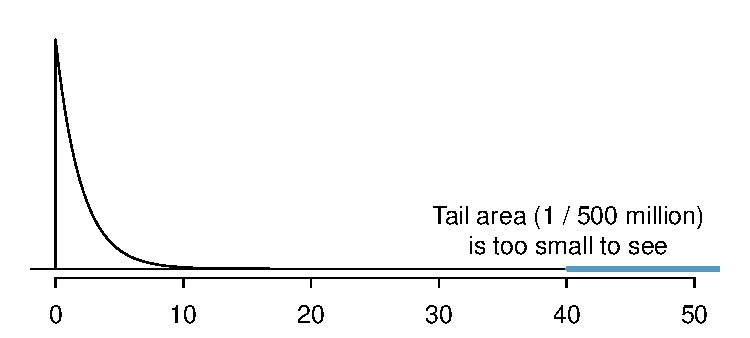
\includegraphics[width=0.65\textwidth]{ch_inference_for_props/figures/iPodChiSqTail/iPodChiSqTail}
\caption{Visualization of the p-value for $X^2 = 40.13$
    when $df = 2$.}
\label{iPodChiSqTail}
\end{figure}

\begin{examplewrap}
\begin{nexample}{Find the p-value and draw a conclusion
    about whether the question affects the sellers likelihood
    of reporting the freezing problem.}
  % Looking in Appendix~\ref{chiSquareProbabilityTable}
  % on page~\pageref{chiSquareProbabilityTable},
  % we examine the row corresponding to 2 degrees of freedom.
  % The test statistic, $X^2 = 40.13$,
  % is larger than the value in the last column,
  % meaning the tail area and p-value are smaller than 0.001.
  Using a computer, we can compute a very precise value
  for the tail area above $X^2 = 40.13$ for a chi-square
  distribution with 2 degrees of freedom:
  0.000000002.
  (If using the table in
    Appendix~\ref{chiSquareProbabilityTable},
    we would identify the p-value is smaller
    than 0.001.)
  Using a significance level of $\alpha=0.05$,
  the null hypothesis is rejected since the p-value is smaller.
  That is, the data provide convincing evidence that the
  question asked did affect a seller's likelihood to tell
  the truth about problems with the iPod.
\end{nexample}
\end{examplewrap}

\index{data!iPod|)}

\index{data!diabetes|(}

\begin{examplewrap}
\begin{nexample}{Figure~\ref{diabetes2ExpMetRosiLifestyleSummary}
    summarizes the results of an experiment evaluating
    three treatments for Type~2 Diabetes in patients
    aged 10-17 who were being treated with metformin.
    The three treatments considered were
    continued treatment with metformin (\resp{met}),
    treatment with metformin combined with rosiglitazone
    (\resp{rosi}),
    or a lifestyle intervention program.
    Each patient had a primary outcome, which was either lacked
    glycemic control (failure)
    or did not lack that control (success).
    What are appropriate hypotheses for this test?}
  \label{diabetes2ExpMetRosiLifestyleIntroExample}
  \begin{itemize}
  \item[$H_0$:] There is no difference in the effectiveness
      of the three treatments.
  \item[$H_A$:] There is some difference in effectiveness
      between the three treatments, e.g. perhaps the
      \resp{rosi} treatment performed better than
      \resp{lifestyle}.
  \end{itemize}
\end{nexample}
\end{examplewrap}

\begin{figure}[h]
\centering
\begin{tabular}{l ccc l}
\hline
 & Failure & Success & Total \\ 
\hline
\resp{lifestyle} & 109 & 125 & 234 \\ 
\resp{met} & 120 & 112 & 232 \\ 
\resp{rosi} &  90 & 143 & 233 \\ 
\hline
Total & 319 & 380 & 699 \\
\hline
\end{tabular}
\caption{Results for the Type~2 Diabetes study.}
\label{diabetes2ExpMetRosiLifestyleSummary}
\end{figure}

\D{\newpage}

\begin{exercisewrap}
\begin{nexercise}
A chi-square test for a two-way table may be used to test
the hypotheses in
Example~\ref{diabetes2ExpMetRosiLifestyleIntroExample}.
As a first step, compute the expected values for each of the
six table cells.\footnotemark{}
\end{nexercise}
\end{exercisewrap}
\footnotetext{The expected count for
    row one / column one is found by multiplying the
    row one total (234) and column one total (319),
    then dividing by the table total (699):
    $\frac{234\times 319}{699} = 106.8$.
    Similarly for the second column and the first row:
    $\frac{234\times 380}{699} = 127.2$.
    Row 2: 105.9 and 126.1.
    Row 3: 106.3 and 126.7.}

\begin{exercisewrap}
\begin{nexercise}
Compute the chi-square test statistic for the data in
Figure~\ref{diabetes2ExpMetRosiLifestyleSummary}.\footnotemark
\end{nexercise}
\end{exercisewrap}
\footnotetext{For each cell,
    compute $\frac{(\text{obs} - \text{exp})^2}{exp}$.
    For instance, the first row and first column:
    $\frac{(109-106.8)^2}{106.8} = 0.05$.
    Adding the results of each cell gives the
    chi-square test statistic:
    {\scriptsize$X^2 = 0.05 + \cdots + 2.11 = 8.16$}.}

\begin{exercisewrap}
\begin{nexercise}
Because there are 3 rows and 2 columns,
the degrees of freedom for the test is
$df = (3 - 1) \times (2 - 1) = 2$.
Use $X^2 = 8.16$, $df = 2$, evaluate whether
to reject the null hypothesis using a significance level
of~0.05.\footnotemark
\end{nexercise}
\end{exercisewrap}
\footnotetext{
    If using a computer, we can identify the p-value
    as 0.017.
    That is, we reject the null hypothesis because
    the p-value is less than 0.05, and we conclude
    that at least one of the treatments is more or
    less effective than the others at treating
    Type~2 Diabetes for glycemic control.}

\index{data!diabetes|)}

\CalculatorVideos{the chi-square test for independence}


{\exercisesheader{}

% 1

\eoce{\qt{Quitters\label{quitters_chisq_independence}} Does being part of a 
support group affect the ability of people to quit smoking? A county 
health department enrolled 300 smokers in a randomized experiment. 150 
participants were assigned to a group that used a nicotine patch and 
met weekly with a support group; the other 150 received the patch and 
did not meet with a support group. At the end of the study, 40 of the 
participants in the patch plus support group had quit smoking while 
only 30 smokers had  quit in the other group.
\begin{parts}
\item Create a two-way table presenting the results of this study.
\item Answer each of the following questions under the null hypothesis 
that being part of a support group does not affect the ability of 
people to quit smoking, and indicate whether the expected values are 
higher or lower than the observed values.
\begin{subparts}
\item How many subjects in the ``patch + support" group would you 
expect to quit?
\item How many subjects in the ``patch only" group would you expect to 
not quit?
\end{subparts}
\end{parts}
}{}

% 2

\eoce{\qt{Full body scan, Part II\label{full_body_scan_chisq_indep}} The 
table below summarizes a data set we first encountered in 
Exercise~\ref{full_body_scan_HT_Error} regarding views on full-body 
scans and political affiliation. The differences in each political 
group may be due to chance. Complete the following computations under 
the null hypothesis of independence between an individual's party 
affiliation and his support of full-body scans. It may be useful to 
first add on an extra column for row totals before proceeding with the 
computations.
\begin{center}
\begin{tabular}{ll  cc c} 
            &   & \multicolumn{3}{c}{\textit{Party Affiliation}} \\
\cline{3-5}
                                &           & Republican & Democrat & Independent   \\
\cline{2-5}
\multirow{3}{*}{\textit{Answer}}& Should    & 264        & 299      & 351 \\
                                & Should not& 38         & 55       & 77 \\
                                & Don't know/No answer & 16 & 15    & 22 \\
\cline{2-5}
                                & Total      & 318       & 369      & 450
\end{tabular}
\end{center}
\begin{parts}
\item How many Republicans would you expect to not support the use of 
full-body scans?
\item How many Democrats would you expect to support the use of full-
body scans?
\item How many Independents would you expect to not know or not answer?
\end{parts}
}{}

% 3

\eoce{\qt{Offshore drilling, Part III\label{offshore_drilling_chisq_indep}} 
The table below summarizes a data set we first encountered in 
Exercise~\ref{offshore_drill_edu_dontknow_HT} that examines the 
responses of a random sample of college graduates and non-graduates on 
the topic of oil drilling. Complete a chi-square test for these data to 
check whether there is a statistically significant difference in 
responses from college graduates and non-graduates.
\begin{center}
\begin{tabular}{l c c}
			& \multicolumn{2}{c}{\textit{College Grad}} \\
\cline{2-3}
			& Yes		& No				\\
\cline{1-3}
Support		& 154		& 132			\\
Oppose		& 180		& 126			\\
Do not know	& 104		& 131			\\
\cline{1-3}
 Total		& 438		& 389		
\end{tabular}
\end{center}
}{}

% 4

\eoce{\qt{Parasitic worm\label{parasitic_worm_chisq}}
Lymphatic filariasis is a disease caused by a parasitic worm.
Complications of the disease can lead to extreme swelling
and other complications.
Here we consider results from a randomized experiment
that compared three
different drug treatment options to clear people of the
this parasite, which people are working to eliminate entirely.
The results for the second year of the study are
given below:\footfullcite{King_Suamani_2018}
\begin{center}
\begin{tabular}{l cc}
  \hline
  & Clear at Year 2 & Not Clear at Year 2 \\ 
  \hline
  Three drugs & 52 & 2 \\ 
  Two drugs & 31 & 24 \\ 
  Two drugs annually & 42 & 14 \\ 
  \hline
\end{tabular}
\end{center}
\begin{parts}
\item\label{parasitic_worm_chisq_hyp}
    Set up hypotheses for evaluating
    whether there is any difference in the
    performance of the treatments,
    and also check conditions.
\item
    Statistical software was used to run
    a chi-square test, which output:
    \begin{align*}
    &X^2 = 23.7
    &&df = 2
    &&\text{p-value} = \text{7.2e-6}
    \end{align*}
    Use these results to evaluate the hypotheses
    from part~(\ref{parasitic_worm_chisq_hyp}),
    and provide a conclusion
    in the context of the problem.
\end{parts}
}{}
}
